\documentclass[11pt]{article}

\usepackage[a4paper,margin=1in]{geometry}
\usepackage[T1]{fontenc}
\usepackage[utf8]{inputenc}
\usepackage{lmodern}
\usepackage[final]{microtype}

\usepackage{amsmath, amssymb, mathtools}
\usepackage{bm}
\usepackage{booktabs}
\usepackage{longtable}
\usepackage{tabularx}
\usepackage{array}
\usepackage{multirow}
\IfFileExists{siunitx.sty}{%
  \usepackage{siunitx}
  \sisetup{detect-all=true}
}{%
  \newcolumntype{S}{>{\raggedleft\arraybackslash}r}
  \providecommand{\sisetup}[1]{}
}
\usepackage{enumitem}
\usepackage{fancyvrb}
\usepackage{graphicx}
\usepackage{xcolor}
\usepackage{tikz}
\usepackage{pgfplots}
\pgfplotsset{compat=1.18}
\usetikzlibrary{positioning, shapes.geometric, arrows.meta, calc, backgrounds, fit, decorations.pathmorphing}
\usepackage{caption}
\usepackage{subcaption}
\captionsetup{font=small, labelfont=bf, format=plain, justification=justified}

\definecolor{abelblue}{HTML}{4E79A7}
\definecolor{abelorange}{HTML}{F28E2B}
\definecolor{abelred}{HTML}{E15759}
\definecolor{abelteal}{HTML}{76B7B2}
\definecolor{abelgreen}{HTML}{59A14F}
\definecolor{abelyellow}{HTML}{EDC948}
\definecolor{abelpurple}{HTML}{B07AA1}
\definecolor{abelpink}{HTML}{FF9DA7}
\definecolor{abelbrown}{HTML}{9C755F}
\definecolor{abelgray}{HTML}{BAB0AC}
\definecolor{abeldark}{HTML}{2E2E2E}

\pgfplotsset{
  every axis/.append style={
    line width=0.6pt,
    tick style={line width=0.5pt, color=abeldark!70},
    grid=major,
    grid style={line width=0.3pt, color=abelgray!50, dashed},
    label style={font=\small},
    tick label style={font=\footnotesize},
    legend style={font=\footnotesize, draw=abeldark!30, fill=white, fill opacity=0.92, text opacity=1, line width=0.5pt},
    cycle list={
      {abelblue, mark=*, mark size=2.5pt, line width=1.2pt},
      {abelorange, mark=triangle*, mark size=2.5pt, line width=1.2pt, dashed},
      {abelred, mark=square*, mark size=2.2pt, line width=1.2pt, dotted},
      {abelteal, mark=diamond*, mark size=2.5pt, line width=1.2pt, densely dashed},
    },
  },
}

\usepackage[hang, flushmargin]{footmisc}
\usepackage[hidelinks]{hyperref}
\usepackage{url}
\usepackage{csquotes}
\usepackage[
  backend=bibtex,
  style=numeric-comp,
  sorting=none,
  maxbibnames=5,
  minbibnames=3,
  giveninits=true,
]{biblatex}

\addbibresource{references.bib}

\hypersetup{
  pdfauthor={Stephen Wang},
  pdftitle={Boundaries of Retail Quantitative Trading on Prediction Markets},
  pdfsubject={Empirical Retrospective on LLM-Assisted Retail Prediction-Market Trading},
  pdfkeywords={prediction markets, LLM trading, ceiling-pin, anchoring bias, abelian methodology, retrospective}
}

\title{\bfseries\Large Boundaries of Retail Quantitative Trading on Prediction Markets:\\
\large A Multi-Mechanism Empirical Retrospective}

\author{
Stephen Wang\thanks{Correspondence: \texttt{lab@abel.ai}.}\\
Abel AI Lab\\
\texttt{lab@abel.ai}
}

\date{May 6, 2026}

\setlist{leftmargin=*}
\setlength{\emergencystretch}{3em}
\sloppy
\makeatletter
\renewcommand*\l@subsection{\@dottedtocline{2}{1.5em}{3.2em}}
\makeatother

\begin{document}
\maketitle

\begin{abstract}
When LLMs meet retail prediction markets, four gates determine whether any route survives: sourceability, fillability, capacity, and anchor stability. We document each gate with concrete evidence from 13 Abel AI Lab campaigns and 156 instrumented adversarial-review rounds in 2026-Q2, identify a cross-mechanism failure mode we name ceiling-pin layer migration --- the LLM-extraction defect that moves from the rubric layer to the prompt layer once the rubric is tightened, observed in n=3 cross-mechanism instances (llm-narrative-trade-0125, llm-deploy-10k, path-c-1week-probe) --- and formalize a pre-launch program-gate methodology that caught 18 of 21 launch defects before any implementation round began. The corpus combines 12 fully instrumented Abelian campaigns, one peer-files-only active campaign, and four sparse legacy inventories retained for denominator honesty but excluded from active analysis. We preserve 225 alternative routes with their selected, rejected, deferred, and promoted decisions, a 52-row strict-parsed attack registry, a 40-quote verbatim evidence bank, and a methodology timeline distinguishing pre-registered from retrospectively analyzed campaigns. The methodology contribution is the empirical record of Abelian rule \#16 R0 gates: Path C narrowed 18 to 3 to 1 to 0 attacks, while Paper 2 narrowed 21 to 6 to 4 to 3 to 1 before R1 extraction. The sister MarketAnchor v0.1.2 result contributes only the narrower observation that consensus-anchor sensitivity exists in one stored LLM forecasting run, with mean net signed drift of 256.73 probability bps; it is not cited as tradable edge, return, or calibration error. The contribution is a map of failure modes for retail builders, a methodology that generalizes beyond trading, and a failure-preserving corpus for cross-validation. The claim is bounded: single-lab, single-period; suggestive, not structural. The repository and Zenodo DOI are planned for public release after Abel AI Lab license confirmation. MarketAnchor v0.1.2 remains citation pending verification until an external identifier exists.
\end{abstract}

\section*{Foreword from Abel AI Lab}
Abel AI Lab studies autonomous research systems when they touch real markets, real code, and real institutional constraints rather than toy tasks. The lab's operating premise is simple: AI systems become useful when they survive measurement, adversarial critique, and operational accountability.

This paper maps a boundary. It is not a product launch note and not a trading signal sheet. It records what happened when Abelian research loops repeatedly tried to turn LLM-accessible market information into deployable prediction-market strategies.

The object of study is deliberately narrow. Stephen Wang ran the campaigns at Abel AI Lab during 2026-Q2, with Claude and Codex used as adversarial research tools under a human-authored program contract. The aim is open knowledge sharing on LLM-trading boundaries: null results, broken gates, and capacity ceilings belong in the record.

MarketAnchor v0.1.2 is the sister paper to this retrospective. It isolates consensus-anchor sensitivity in a stored prediction-market forecasting run and is cited here only for that narrower construct. Its SHA256 is preserved as 8968953708979dc2bd2915ec5c0a22c40e730c24d8134470739b7084bec5ca27.

The roadmap continues from this paper. MarketAnchor v0.2 will test anchor controls more directly, and the smart-money signal program will ask whether external participant behavior can become a grounded signal without borrowing unsupported authority from LLM priors.

The lab does not treat LLMs as authors. Claude and Codex contributed critique, extraction, drafting assistance, and verification pressure. The human author owns the decisions, the claims, and the release.

The manuscript is also a lab-process artifact. It puts the empirical trading boundary and the methodology boundary in one place, for researchers, traders, and builders who do not want to spend weeks rediscovering the same constraints.

The standard for this draft is goal-driven evidence rather than eval-gaming. Every retained claim advances the mechanism map, marks a limitation, or preserves provenance for reviewers who want to attack the record directly.

The contribution is a first systematic empirical retrospective, not a universal theorem. The evidence is single-lab and single-period, but unusually dense in adversarial review artifacts. Abel AI Lab releases this draft to keep those artifacts legible.

\section*{AI and Tool Assistance Disclosure}
Anthropic Claude was used for peer-challenge critique, framing review, and cross-attack peer policy in adversarial review rounds. OpenAI Codex CLI gpt-5.5, reasoning effort xhigh, was used for repository inspection, statistical recomputation support, deep transcript mining across peer files, data-quality repair, verified arXiv reference checks, and section drafting assistance. The human author reviewed all outputs and accepts responsibility for the manuscript, statistics, code references, citations, and claims. These tools are not authors.

\tableofcontents

\section{Introduction}
\label{sec:introduction}
This paper is the first systematic empirical map of a narrow but economically important question: what happens when modern LLM agents are repeatedly aimed at retail-scale prediction-market trading under adversarial review?

The question matters because prediction markets expose public prices, open settlement rules, and fragmented liquidity in a form that looks unusually accessible to language models. A model can read a market title, a rule page, a news article, an order book snapshot, and a prior campaign memo inside one working context.

That accessibility creates an obvious temptation. If an LLM can summarize rules, surface event evidence, and propose trades faster than a human retail operator, then perhaps the remaining problem is just engineering throughput.

The campaigns studied here tested that temptation in practice. They looked for threshold-ladder arithmetic, duplicated-market relationships, date-ladder monotonicity, cross-platform price gaps, internal-feature residuals, LLM narrative priors, event-contract rule extraction, and SEC special-situation extraction.

The result is not a single failure. It is a pattern of boundary conditions. Some mechanisms die because public markets already absorbed them. Some die because the book is too thin. Some die because the LLM can fill a rubric without grounding the field. Some die because the measured prior is not independent of the prompt-visible consensus.

Null results matter in this domain because trading literature is prone to survivorship bias. Failed mechanisms disappear from public memory, while backtests that once worked remain named and reusable long after the live market changed.

The Abelian corpus is useful because it preserves the failure trail. Peer files record objections before the operator can round them away. Mission threads preserve rejected routes as data. Eval logs separate score movement from profit movement. Program gates show when a research plan was too vague to launch.

The paper therefore treats the archive as an empirical object. The unit is not only a trade or a backtest row. It is a round in which an LLM-assisted system proposed a route, mutated code or prose, received adversarial critique, and either moved a metric or exposed a blocker.

The active corpus is 13 campaigns and 156 instrumented rounds. The raw inventory is 17 campaigns and 164 round directories, but four legacy directories contain no transcript files and are retained only for inventory completeness.

The analyzed period is a 12-calendar-day window ending on 2026-05-05, with active instrumented campaign work concentrated in four active days from 2026-05-02 through 2026-05-05. This distinction matters because calendar span and active execution span are not the same measure.

The trading subset is smaller than the corpus headline. Core infrastructure accounts for 97 rounds from pm-live-readiness and ws-cron-alignment. Cron-fill-grounded-truth adds 5 adjacent infrastructure rounds and is counted in the trading-focused remainder only when its evidence directly bears on mechanism saturation.

The paper uses 59 trading-focused rounds across 11 active trading campaigns for the substantive findings. Infrastructure rounds contribute to methodology and to safety/freshness constraints, not as direct evidence of profitable trading mechanisms.

The four findings are intentionally framed as observed boundaries. Math-arbitrage saturation describes mechanisms that were valid historically or locally but closed under current Polymarket conditions. The LLM-extraction ceiling-pin describes confidence or rubric systems that reach high scores without adding tradeable truth. The capacity ceiling describes the economics of small books and fee floors. Anchoring uncertainty describes how prompt-visible consensus contaminates claimed independent priors.

The paper does not claim that prediction markets are efficient in every niche. It reports that in this lab's 2026-Q2 campaigns, the obvious LLM-accessible retail routes did not produce durable greater-than-\$1k-per-month edge after adversarial review.

The scope is also not a complete taxonomy of quantitative trading. The campaigns are Stephen-curated, the operator is one person, and the tooling stack reflects Abel AI Lab's preferences. Those limitations make the map descriptive rather than universal.

The value of the map is still practical. A builder considering a similar path can inspect which ideas failed for data-quality reasons, which failed for economics, which failed for LLM grounding, and which remain plausible only after new controls.

The paper structure follows the empirical path. Section 2 situates the work against LLM forecasting, financial LLMs, prediction-market studies, and anchoring literature. Section 3 defines the corpus and methodology. Sections 4 through 7 present the four findings. Section 8 extracts the Abelian methodology contribution.

Discussion, limitations, and open problems are treated as part of the empirical result, not as back matter. They state where the evidence stops, which mechanisms remain plausible, and which follow-on programs would actually test the next claim.

\section{Related Work}
\label{sec:related-work}
The nearest literature already knows how to ask LLMs for forecasts; this paper asks what breaks when those forecasts become candidate trades. ForecastBench (\cite{Karger2024ForeDyna}) builds a dynamic benchmark for open-domain AI forecasting, so it is directly relevant to whether a model can emit useful probabilities about unresolved events. Prophet Arena (\cite{Yang2025LlmAs}) asks a related predictive-intelligence question and uses prediction-market performance as part of the comparison surface. AI-Augmented Predictions (\cite{Schoenegger2024AiAugm}) studies LLMs as forecasting assistants for humans rather than autonomous capital-allocation systems. LiveTradeBench (\cite{Yu2025LiveSeek}) moves closer to trading by using live market data, while Pratt et al.'s forecasting-strategy study (\cite{Pratt2024CanLang}) tests whether language models can apply named forecasting heuristics rather than merely produce fluent rationales.

That forecasting strand contributes benchmark design, task construction, probability elicitation, and evidence that LLMs can sometimes help forecasters. It does not by itself answer what happens when a probability becomes a route to order placement. Other temporal forecasting work expands the benchmark context: temporal-event evaluation (\cite{Chang2024CompEval}), time-series prompting through AutoTimes (\cite{Liu2024AutoAuto}), PROPHET-style future forecasting (\cite{Tao2025PropInfe}), multimodal event forecasting (\cite{Li2024MmFore}), and macroeconomic forecasting with LLMs (\cite{Carriero2024MacrFore}) all widen the set of domains in which forecast quality can be measured. Paper 2 is not a forecasting benchmark. It studies what happens when LLM forecasters are treated as trading routes under adversarial review, where the failure mode includes ceiling-pin defects in field extraction, source grounding, and capacity, not only forecast inaccuracy.

The anchoring literature intersects forecasting at the point where a probability is no longer merely an answer, but a response to visible context. Lou and Sun (\cite{Lou2024AnchBias}) directly study anchoring bias in large language models. SynAnchors (\cite{Huang2025UndeAnch}) pushes further into mechanism and mitigation by constructing synthetic data to isolate the anchoring effect. Sharma et al. (\cite{Sharma2023TowaUnde}) frame sycophancy as agreement with user beliefs or prompt pressure, and Wei et al. (\cite{Wei2023SimpSynt}) show that synthetic data can reduce such behavior. Perez et al.'s model-written evaluation work (\cite{Perez2022DiscLang}), the InstructGPT RLHF paradigm (\cite{Ouyang2022TraiLang}), Constitutional AI (\cite{Bai2022ConsAi}), and calibration-oriented language-model behavior work (\cite{Kadavath2022LangMode}) give the broader alignment-era context in which assistant models are trained to be helpful, preference-aware, and sometimes overly compliant.

Paper 2 uses that literature narrowly. It does not make a general model-behavior claim about all LLM anchoring or sycophancy. Section 7 invokes the sister MarketAnchor v0.1.2 result only for consensus-anchor sensitivity in one stored prediction-market forecasting run: 256.73 probability basis points of mean net signed drift. That statistic is not tradable edge, not return, not calibration error, not forecast accuracy, and not trading profit. Paper 2's separate trading-operational claim is that any LLM-prior trading edge below roughly 500 bps is contaminated unless anchor controls are applied when the prior was elicited near market consensus. The contribution is a trading-system hygiene rule, not a new taxonomy of model psychology.

Financial-LLM work supplies the agent and domain-specialization backdrop, but not the retail prediction-market boundary by itself. BloombergGPT (\cite{Wu2023BlooLarg}) shows the value of finance-tuned language modeling at scale. FinGPT (\cite{Yang2023FingOpen}) and the related data-democratization work (\cite{Liu2023FingDemo}) make the case for open finance LLM infrastructure. FinTral (\cite{Bhatia2024FintFami}) extends finance LLMs into multimodal settings. FinLLM-B (\cite{Zhang2024FinlB}) evaluates LLMs for breakout trading. StockAgent (\cite{Zhang2024WhenAi}), TradingAgents (\cite{Xiao2024TradMult}), and market-simulation work on LLM trading agents (\cite{LopezLira2025CanLarg}) study agent behavior in financial decision loops.

That strand contributes model specialization, agent architecture, market-simulation protocols, and the claim that LLMs can participate in financial workflows. Paper 2 complements it with a narrower negative map: on prediction markets specifically, at retail bankroll scale, the obvious LLM-accessible routes in this Abel AI Lab corpus did not produce a sustainable greater-than-\$1k-per-month edge after adversarial review. The diagnosis is not that finance LLMs are useless. It is that public market information, rule text, and prompt priors can be easy for many participants to access, while the remaining edge is eroded by source-grounding, fee, fillability, and capacity gates.

That positive finance-LLM backdrop needs the older financial-ML critique beside it. \textcite{Lo2002StatisticsSharpeRatios} shows that a reported Sharpe ratio is a statistic with distributional and serial-correlation assumptions, not a standalone proof of edge. \textcite{Bailey2014DeflatedSharpeRatio} formalize the deflated Sharpe ratio to correct for selection bias, non-normality, and multiple trials. \textcite[Chs.~11--12]{LopezDePrado2018AdvancesFinancialMachineLearning} turns that critique into workflow guidance: backtests are research artifacts vulnerable to overfitting unless the validation design accounts for the search process. Paper 2 imports that caution at the route level: an LLM-generated idea is not promoted because the local score rose; it is promoted only if the source, time, fill, and capacity gates survive.

Prediction-market-specific work brings the evaluation surface closest to the campaigns studied here. The canonical social-science base predates the current LLM benchmark wave: \textcite{Wolfers2004PredictionMarkets} survey prediction markets as information-aggregation mechanisms, \textcite{Manski2006InterpretingPredictionMarkets} warns that market prices do not mechanically identify a mean belief without assumptions about preferences and wealth, and \textcite{Snowberg2010FavoriteLongshotBias} show that favorite-longshot bias can distort the interpretation of market-implied probabilities. Those references matter here because Paper 2 treats prices as execution constraints and consensus anchors, not as ground truth.

The newer prediction-market LLM work then supplies the direct comparison set. PolyBench (\cite{Cheng2026PolyBenc}) proposes a Polymarket benchmark for LLM forecasting and trading capabilities on live prediction-market data. LiveTradeBench (\cite{Yu2025LiveSeek}) is adjacent because it also treats market data as an evaluation substrate. PolySwarm (\cite{Barot2026PolyMult}) studies multi-agent prediction-market trading and latency arbitrage, focusing on emergent behaviors when multiple LLM agents interact with the same order book. Paper 2 differs in three ways: (a) single-operator retail bankroll rather than multi-agent simulation; (b) failure-preserving retrospective rather than benchmark scoring; and (c) a cross-mechanism ceiling-pin diagnosis spanning LLM-extraction failure modes that PolySwarm's interaction-focused frame does not directly probe. Polymarket order-book microstructure evidence (\cite{Dubach2026AnatDece}), 2024 election-market anatomy (\cite{Tsang2026AnatPoly}), prediction-market arbitrage structure (\cite{Saguillo2025UnraProb}), and UMA-resolved Polymarket dispute arbitration (\cite{Wen2026CanLlms}) define the market context in which this paper's campaigns operated.

Classic market microstructure explains why that market context cannot be reduced to a probability table. \textcite{Glosten1985BidAskTransactionPrices} give the adverse-selection account of bid, ask, and transaction prices when informed and uninformed traders meet through a specialist. \textcite{Easley1996LiquidityInformation} connect liquidity and information to infrequently traded securities, a close conceptual match to thin prediction-market books. \textcite{Stoll1989BidAskSpreadComponents} decomposes the bid-ask spread into inventory, order-processing, and adverse-information components. Section 6 uses those ideas operationally: a quoted edge is not a deployable edge unless the spread, depth, inventory risk, and information asymmetry leave enough capacity after fees.

Those papers are useful context, but the object differs. Paper 2 is not a benchmark proposal and does not score models on a public leaderboard. It uses prediction-market campaigns as an empirical retrospective object. The evidence comes from internal Abelian campaign logs, state files, peer attacks, quote banks, and route registries. PolyBench and LiveTradeBench matter because they show that the subfield is converging on live prediction-market data as a serious evaluation ground. Paper 2 contributes the complementary artifact: a failure-preserving map of what happened when one lab tried to turn that data into retail trading operations.

Survivorship bias and false-positive control supply the final lens because trading failures usually vanish before they become evidence. \textcite{Brown1992SurvivorshipBias} show how performance studies can be distorted when failed funds disappear from the sample. \textcite{Harvey2016CrossSectionExpectedReturns} make the factor-zoo problem explicit: once enough candidate signals are tried, conventional thresholds are no longer credible evidence of expected return. \textcite{Bailey2014DeflatedSharpeRatio} add the deflated Sharpe ratio as a correction for selection, backtest overfitting, and non-normal returns, while \textcite{Lo2002StatisticsSharpeRatios} shows why Sharpe ratio inference itself depends on the return process. \textcite[Ch.~11]{LopezDePrado2018AdvancesFinancialMachineLearning} concentrates the warning in financial-machine-learning terms: even a flawless-looking backtest can be wrong if it is a product of the search procedure.

Paper 2 does not try to settle that literature. It uses the warning operationally: failed campaigns are preserved as data, not omitted as embarrassing dead ends. The relevant unit is not only a profitable row; it is the route that was proposed, attacked, narrowed, rejected, or quarantined before money could scale. That design is intentionally hostile to survivorship. The 4 sparse legacy inventories remain in the denominator, the 13 active campaigns are separated from the 17 raw directories, the R2 eval-gaming failure is preserved as a methodology lesson, and promoted routes are reported beside rejected and deferred routes.

That operational use is methodologically important for the LLM-trading subfield. Most agent papers naturally emphasize successful trajectories, benchmark scores, or simulations that finish with a model-comparison table. This paper keeps R0 refusals, peer attacks, route rejections, ceiling-pin failures, and eval-gaming repairs in the empirical record. The null result is therefore not a blank outcome. It is a structured account of which routes failed at which gate, with the same archive also preserving the few routes that remained plausible only after tighter controls.

Across the five strands, the distinct contribution is therefore specific. Paper 2 does not claim a universal limit on prediction-market efficiency, a universal limit on LLM trading, or a new general theory of anchoring. It contributes the first Abel AI Lab multi-campaign retrospective of LLM-assisted retail prediction-market trading attempts: 13 active campaigns, 156 instrumented rounds, explicit corpus exclusions, source-grounding evidence, capacity analysis, anchor-control implications, and an Abelian methodology record that keeps failed routes available for audit.

\begin{center}
\scriptsize
\setlength{\tabcolsep}{1.5pt}
\renewcommand{\arraystretch}{1.18}
\begin{longtable}{@{}>{\raggedright\arraybackslash}p{0.095\textwidth}>{\raggedright\arraybackslash}p{0.120\textwidth}>{\raggedright\arraybackslash}p{0.130\textwidth}>{\raggedright\arraybackslash}p{0.130\textwidth}>{\raggedright\arraybackslash}p{0.145\textwidth}>{\raggedright\arraybackslash}p{0.115\textwidth}>{\raggedright\arraybackslash}p{0.145\textwidth}@{}}
\caption{Comparison with adjacent prediction-market and LLM-trading benchmark literature.}
\label{tab:related-work-comparison}\\
\toprule
\textbf{Paper or benchmark} & \textbf{Substrate} & \textbf{Object of study} & \textbf{Failure preservation} & \textbf{Methodology contribution} & \textbf{Lab structure} & \textbf{Quantitative outcome} \\
\midrule
\endfirsthead
\toprule
\textbf{Paper or benchmark} & \textbf{Substrate} & \textbf{Object of study} & \textbf{Failure preservation} & \textbf{Methodology contribution} & \textbf{Lab structure} & \textbf{Quantitative outcome} \\
\midrule
\endhead
Paper 2 & Abel AI Lab campaign archive plus Polymarket/\allowbreak Kalshi-adjacent route evidence. & Retail LLM-assisted prediction-market trading attempts under adversarial review. & High: R0 refusals, rejected routes, ceiling-pins, and eval-gaming repairs remain in the corpus. & Failure-preserving retrospective with route gates for sourceability, fillability, capacity, and anchoring. & Single-lab, single-operator, single-period. & 13 active campaigns, 156 instrumented rounds, n=3 ceiling-pin observations, and no durable greater-than-\$1k-per-month route. \\
PolyBench (\cite{Cheng2026PolyBenc}) & Live Polymarket data packaged as an LLM benchmark substrate. & LLM forecasting and trading capability on prediction-market tasks. & Benchmark-oriented: failures appear through model scores rather than preserved campaign archaeology. & Public task construction for live prediction-market evaluation. & Benchmark paper, not this lab's retrospective corpus. & Quantitative outcome is model-performance benchmarking, not a single-operator PnL boundary. \\
LiveTrade\-Bench (\cite{Yu2025LiveSeek}) & Live market data for real-world alpha-seeking evaluation. & Whether LLM agents can seek trading alpha in live settings. & Partial: failed predictions can be scored, but the paper is not built around retained route refusals. & Moves evaluation from static finance QA toward live trading substrates. & External benchmark setting rather than Abel AI Lab's single-operator archive. & Quantitative outcome is benchmark performance, not failure-preserved route attrition. \\
Prophet Arena (\cite{Yang2025LlmAs}) & Prediction-market-linked forecasting arena. & Predictive intelligence of LLMs across unresolved events. & Low-to-medium: the emphasis is arena comparison, not rejected-trade provenance. & Treats prediction-market performance as an evaluation signal for forecasting intelligence. & Multi-model arena framing, not a single-lab trading campaign. & Quantitative outcome is arena/model comparison, not deployable capacity or after-fee execution. \\
\bottomrule
\end{longtable}
\end{center}

\section{Empirical Setting and Methodology}
\label{sec:empirical-setting-and-methodology}
The evidence base is small by lab count and unusually dense by audit trail. The Abelian run registry yields 13 active campaigns and 156 instrumented rounds. The raw inventory contains 17 campaigns and 164 round directories, but four sparse legacy campaigns contain empty round directories and are excluded from active analysis.

The active campaign set consists of 12 fully instrumented campaigns with state files plus peer artifacts and one peer-files-only active campaign. The instrumentation enum in \texttt{cross-campaign-aggregate.json} is restricted to full\_state\_json, peer\_files\_only, and empty\_legacy, which keeps a thin legacy directory from masquerading as a campaign with round-level evidence.

The active execution span is four active days inside a 12-calendar-day window. The earliest active campaign directory is 2026-05-02, and the final R1/R2 paper artifacts are dated 2026-05-05 and 2026-05-06.

Infrastructure dominates the round count, so the paper separates operational hardening from trading evidence before drawing mechanism claims. Core infrastructure accounts for 97 of 156 instrumented rounds: pm-live-readiness contributes 57 rounds and ws-cron-alignment contributes 40 rounds. Cron-fill-grounded-truth contributes 5 adjacent infrastructure rounds and is discussed separately when it bears on mechanism evidence.

The trading-focused empirical record is therefore 59 rounds across 11 active trading campaigns. This paper uses that partition to avoid treating infrastructure hardening as direct trading evidence.

R2 repaired the R1 attack registry because a noisy failure archive is only a different kind of false precision. The old heuristic registry had 3,719 rows and counted transcript noise, route bullets, pass lines, and raw Codex diffs. The repaired registry admits only formal attack blocks with explicit nearby severity and line spans.

Paper 2 self-attacks are quarantined into \texttt{methodology-self-attacks.jsonl}. They remain useful evidence for the methodology contribution but no longer enter cross-campaign recurrence counts.

R2 also rebuilt the quote bank so every quote appears verbatim in its cited source file at its stated line range. The bank is capped by campaign and peer role, preventing one dense infrastructure campaign from dominating the manuscript's textual evidence.

Alternative routes are now split into est\_metric\_delta\_value and est\_metric\_delta\_raw. Numeric estimates are floats only when the source row gave an explicit numeric value; qualitative strings remain raw text with source-file and source-line provenance.

The methodology timeline records the first observed R0 program gate at 2026-05-04T01:01:07Z and separates retrospective campaigns from later pre-launch program-gated campaigns.

The provenance boundary is explicit. It states what the paper uses as trading evidence, what it uses as methodology evidence, and what it quarantines as self-review.

A route is treated as live only after the evidence chain reaches sourceability, fillability, capacity, and post-fee economics. A language model can accelerate the search through that chain, but it does not remove any link from the chain.

Figure~\ref{fig:four-gate-funnel} summarizes that sequence as a four-gate filter.

\begin{figure}[t]
\centering
\resizebox{0.95\textwidth}{!}{%
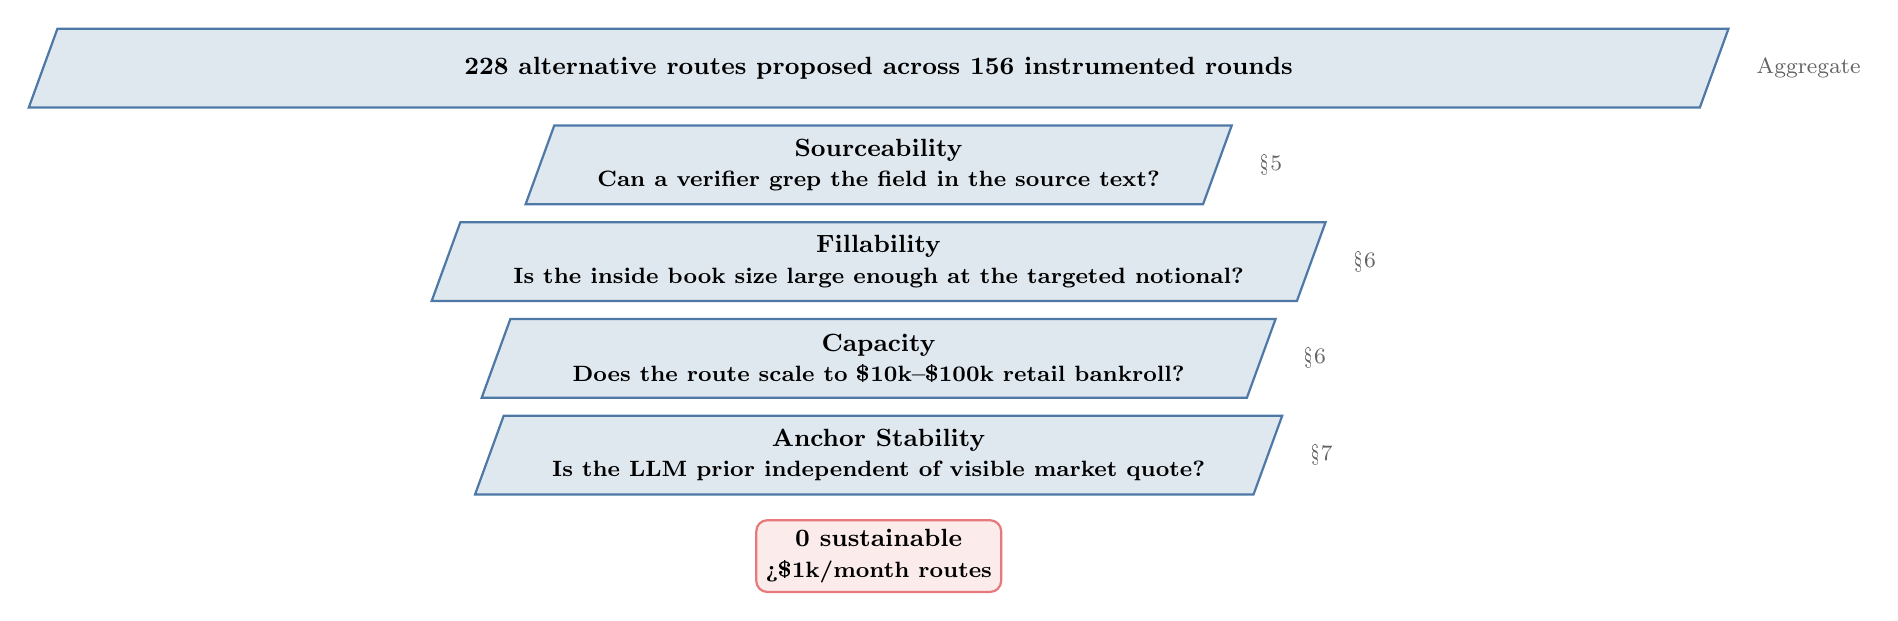
\begin{tikzpicture}[
  gate/.style={
    trapezium, trapezium left angle=70, trapezium right angle=110,
    draw=abelblue, thick, fill=abelblue!18, minimum width=0pt,
    align=center, font=\small\bfseries
  },
  arrow/.style={-Latex, thick, color=abeldark!70},
]
\node[gate, minimum width=10cm, minimum height=1cm] (top)
  {228 alternative routes proposed across 156 instrumented rounds};

\node[gate, minimum width=8.5cm, minimum height=1cm, below=2mm of top]
  (g1) {\textbf{Sourceability}\\\footnotesize{Can a verifier grep the field in the source text?}};

\node[gate, minimum width=7cm, minimum height=1cm, below=2mm of g1]
  (g2) {\textbf{Fillability}\\\footnotesize{Is the inside book size large enough at the targeted notional?}};

\node[gate, minimum width=5.5cm, minimum height=1cm, below=2mm of g2]
  (g3) {\textbf{Capacity}\\\footnotesize{Does the route scale to \$10k--\$100k retail bankroll?}};

\node[gate, minimum width=4cm, minimum height=1cm, below=2mm of g3]
  (g4) {\textbf{Anchor Stability}\\\footnotesize{Is the LLM prior independent of visible market quote?}};

\node[draw=abelred!80, fill=abelred!12, thick, rounded corners,
      minimum width=3cm, minimum height=0.9cm, below=3mm of g4,
      align=center, font=\small\bfseries]
  (bot) {0 sustainable\\\footnotesize{>\$1k/month routes}};

\node[right=4mm of top, font=\footnotesize, color=abeldark!75] {Aggregate};
\node[right=4mm of g1, font=\footnotesize, color=abeldark!75] {\S5};
\node[right=4mm of g2, font=\footnotesize, color=abeldark!75] {\S6};
\node[right=4mm of g3, font=\footnotesize, color=abeldark!75] {\S6};
\node[right=4mm of g4, font=\footnotesize, color=abeldark!75] {\S7};
\end{tikzpicture}
}
\caption{Four-gate filter for retail LLM-assisted prediction-market trading routes. Each gate drops candidate routes that cannot prove the named property at the targeted bankroll. Of 228 alternative routes proposed across 156 instrumented Abelian rounds, no route surveyed in this corpus produced sustainable greater-than-\$1k/month edge after all four gates apply. Section references show where each gate is empirically grounded.}
\label{fig:four-gate-funnel}
\end{figure}

\subsection{Routes Considered Map}
\label{subsec:routes-considered-map}
The alternative-route corpus is where the retrospective stops being a winner's diary. It records paths the agents considered and did not take. The aggregate campaign table counts 228 proposed alternative routes across 156 instrumented rounds. The recovered JSONL registry contains 225 individual route rows: 45 selected, 135 rejected, and 45 deferred. The rejection rate is therefore 59.2\% using the aggregate denominator and 60.0\% using recovered registry rows.

Figure~\ref{fig:alternative-routes-flow} shows the route-decision breakdown preserved by that registry.

Promotion is also informative because it shows what the loop found worth carrying forward, not only what it killed. The aggregate table counts 82 routes promoted to subsequent rounds; the recovered route registry contains 79 promoted rows. Keyword coding of those 79 promoted rows shows 10 evidence, source, filing, or grounding routes; 16 prior, quote, anchor, ablation, or consensus routes; and 39 capacity, backtest, depth, fill, fee, spread, settlement, or PnL routes. Those categories match the four empirical findings rather than forming a separate appendix-only story.

\begin{table}[t]
\caption{Recovered route-registry decision counts.}
\label{tab:route-registry-decisions}
\centering
\small
\begin{tabular}{@{}lSS@{}}
\toprule
\textbf{Decision} & {\textbf{Rows}} & {\textbf{Share (\%)}} \\
\midrule
Selected & 45 & 20.0 \\
Rejected & 135 & 60.0 \\
Deferred & 45 & 20.0 \\
\midrule
Total non-overlap & 225 & 100.0 \\
Promoted overlap & 79 & {} \\
\bottomrule
\end{tabular}
\end{table}

\begin{figure}[t]
\centering
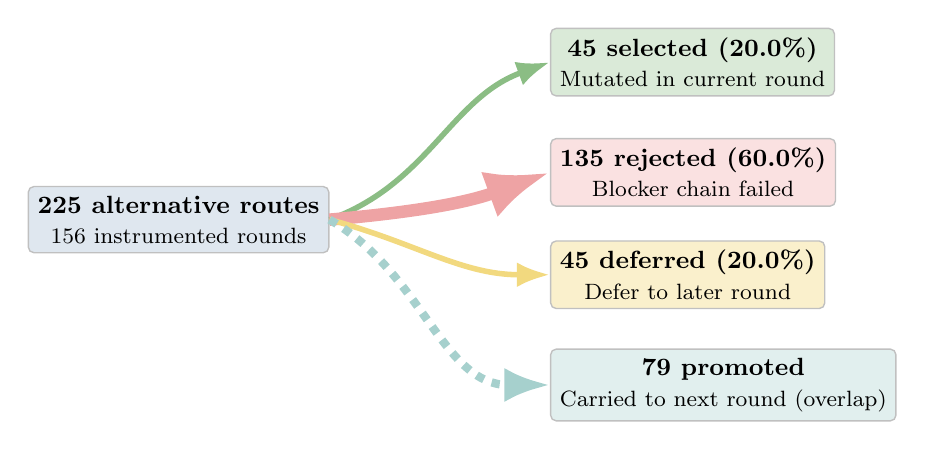
\begin{tikzpicture}[
  node distance=4mm,
  flow/.style={rectangle, rounded corners=2pt, font=\small, align=center, minimum height=0.8cm, draw=abeldark!30, line width=0.5pt},
  arrow/.style={-Latex, color=abelgray!70, line width=0.5pt},
]
\node[flow, fill=abelblue!18, minimum width=3cm] (source) {\textbf{225 alternative routes}\\\footnotesize{156 instrumented rounds}};

\node[flow, fill=abelgreen!22, minimum width=3.2cm, right=2.8cm of source, yshift=2cm] (sel)
  {\textbf{45 selected (20.0\%)}\\\footnotesize{Mutated in current round}};
\node[flow, fill=abelred!18, minimum width=3.2cm, right=2.8cm of source, yshift=0.6cm] (rej)
  {\textbf{135 rejected (60.0\%)}\\\footnotesize{Blocker chain failed}};
\node[flow, fill=abelyellow!28, minimum width=3.2cm, right=2.8cm of source, yshift=-0.7cm] (def)
  {\textbf{45 deferred (20.0\%)}\\\footnotesize{Defer to later round}};
\node[flow, fill=abelteal!22, minimum width=3.2cm, right=2.8cm of source, yshift=-2.1cm] (prom)
  {\textbf{79 promoted}\\\footnotesize{Carried to next round (overlap)}};

\draw[arrow, line width=2.0pt, color=abelgreen!70] (source.east) to[out=20, in=200] (sel.west);
\draw[arrow, line width=4.5pt, color=abelred!55] (source.east) to[out=5, in=200] (rej.west);
\draw[arrow, line width=2.0pt, color=abelyellow!70] (source.east) to[out=-15, in=180] (def.west);
\draw[arrow, line width=3.0pt, color=abelteal!65, dashed] (source.east) to[out=-30, in=180] (prom.west);
\end{tikzpicture}
\caption{Alternative-routes registry breakdown. From 225 routes recorded in the recovered registry across 156 instrumented rounds, 45 (20.0\%) were selected, 135 (60.0\%) rejected, and 45 (20.0\%) deferred; 79 routes were also promoted to subsequent rounds (overlapping with selected/rejected/deferred buckets because the same route can pass through multiple campaign rounds). The aggregate campaign table reports a slightly larger denominator (228 proposed, 82 promoted) because some early-round routes were not preserved verbatim in the recovered registry; \S3.1 separates the two counts.}
\label{fig:alternative-routes-flow}
\end{figure}

The most frequently repeated route IDs were not hidden alpha routes. They were process and infrastructure routes: \texttt{baseline-only} appeared in cron-fill-grounded-truth and ws-cron-alignment, \texttt{skip-baseline} appeared in the same two campaigns and was rejected because it violated verify-before-mutate, and \texttt{both-tracks-parallel}, \texttt{lp-rigor-track}, and \texttt{all-three} each appeared twice inside ws-cron-alignment. The repeated lesson was almost mundane: measurement discipline and websocket/LP rigor kept resurfacing because the system could not safely reason about edge until the measurement substrate held still.

The highest numeric rejected estimates in state mission threads make the same point in a sharper form. \texttt{cron-flagged-plus-shard-rotation} estimated +100 but was rejected because it required new sharding logic rather than the cheaper verifier route (\texttt{2026-05-03-0245-ws-cron-alignment/state.json:L89-L104}). \texttt{multi-conn-sharding} also estimated +100 but was deferred behind time-sharded rotation because it required lifecycle, watchdog, and logging refactors (\texttt{2026-05-03-0245-ws-cron-alignment/state.json:L243-L251}). \texttt{hybrid-multi-and-fast-rotation} estimated +100 but was rejected as over-complex once multi-connection coverage alone became the cleaner mechanism (\texttt{2026-05-03-0245-ws-cron-alignment/state.json:L447-L455}). A route can promise maximum metric movement and still lose because its blast radius makes the next failure harder to observe.

The route map therefore supports a path-dependency claim. Most edges were not undiscovered; they were proposed, attacked, and either selected, rejected, deferred, or promoted with a blocker chain. The rejected pile teaches that high nominal metric movement often lost to implementation blast radius, observability risk, or failure to create profit evidence.

\section{Math-Arb Mechanism Saturation}
\label{sec:math-arb-mechanism-saturation}
Math-arbitrage on Polymarket no longer paid at the retail scale tested here. Across the trading-focused corpus, the most mechanical routes were repeatedly narrowed by current-data checks, book-depth checks, settlement checks, and capacity checks.

The threshold-ladder memory gives the cleanest cautionary contrast. A prior arsenal recorded 327 walk-forward trades over 14 months at positive per-leg returns, but the 2026-05-03 current-market query found zero violations across 4,365 live markets in the relevant NBA, tennis, and soccer ladder families.

That contrast is the important empirical shape: a mechanism can be real historically and closed operationally later. The paper treats the 327-trade record as point-in-time evidence, not as forward alpha.

The market-making branch closed in a different way. The ws-cron-alignment campaign's MM sweep tested delta settings against live fill and markout behavior. At 100 bps, 5 of 6 fills lost money; at 200 bps, 0 of 3 were winning; at 300 bps, n=2 was too small to rescue the route.

The peer-B synthesis in the memory file describes adverse markout as 3 to 30 times captured spread and characterizes Polymarket flow as informed enough that vanilla maker-edge did not survive.

The surviving Polymarket math-arb niche was bydate LP-detected ladder arbitrage. Two Trump China visit baskets survived the R37/R38/R39 chain with concrete live feasible price relationships, but their inside size was measured in cents to low double-digit dollars per poll, not institutional deployment size.

Cross-platform-pilot-b added a broader capacity warning. Cross-venue routes can be conceptually attractive, but the observed cycle economics remained bounded by venue access, book depth, and per-cycle capital that was too small to support a \$10k to \$100k retail pool target.

The internal-feature ML memory supplies the parallel market-efficiency result. On liquid Polymarket markets, LGBM models using only market-internal price, volume, momentum, and category features were uniformly below market p\_snap AUC. The order book already incorporated those features.

The shared mechanism is saturation, not impossibility. Public, liquid, mechanically obvious relationships get arbed. Internal features visible to all participants do not become private signal by passing through a model.

This is the saturation result.

The trading-focused campaign count is 11, and 8 of those explored math-arb-class or adjacent market-structure routes. None produced a sustainable greater-than-\$1k-per-month edge after the current-data, fillability, and capacity gates were applied.

The one-row campaign summary makes the good/bad balance explicit. Cron-fill-grounded-truth and ws-cron-alignment are infrastructure-heavy but still contribute math-arb evidence after down-weighting (\texttt{per-campaign-summary.csv:L3-L4}). Cross-platform-pilot-b, profit-search, pm-5k10k-profit, and pm-10k50k-profit are capacity-ceiling rows rather than pure failures (\texttt{per-campaign-summary.csv:L5-L6,L10-L11}). Crypto-pm-probe is the cleanest negative math-arb row because it repeatedly closes on freshness, settlement, and capacity (\texttt{per-campaign-summary.csv:L7}). The result is balanced: the 327-trade arsenal was real historical alpha, bydate LP arb survived with tiny capacity, and cross-platform scans found real but sub-floor cycle economics; vanilla market-making, internal-feature LGBM, and live threshold-ladder violations failed current deployment checks.

The quote bank anchors the saturation claim at the places where the routes actually broke: side-line contradictions, old math-arb-friendly subscriptions, low-n bydate evidence, and websocket health diagnostics. The Evidence Locator appendix keeps the verbatim source rows out of the argument flow while preserving reviewer-auditable provenance.

The practical implication is front-loaded verification. Math-arb work begins with current-data violation counts, book-depth measurement, and settlement/fillability proof. Backtest history alone is insufficient after market-maker incentives or competing bots change the live state.

The claim is deliberately narrow. It does not say that every prediction-market arbitrage is gone. It says the obvious Polymarket retail mechanisms in this corpus either closed, shrank below useful capacity, or required a different external information source.

The saturation claim is strongest when the source campaign reports a live-market falsifier, not merely a peer's preference. For this reason, ladder closure, vanilla market-making markout, bydate LP survival, and internal-feature ML are separated rather than collapsed into a single math-arb verdict.

\section{Cross-Mechanism LLM-Extraction Ceiling-Pin}
\label{sec:cross-mechanism-llm-extraction-ceiling-pin}
The most dangerous LLM trading failure in the corpus was not low confidence. It was false high confidence. The observed ceiling-pin count in this draft is n=3: llm-deploy-10k, path-c-1week-probe, and the in-flight llm-narrative-trade-0125 R3 observation. The claim remains suggestive, not structural. Three instances across one lab and one period justify a mechanism warning; they do not prove that all LLM trading systems share this defect.

We extend the program contract's initial n=2 scope to n=3 by including the in-flight llm-narrative-trade-0125 R3 observation. This was not part of the original campaign goal-met criterion (ii), which focused on llm-deploy and Path C. The upgrade is empirically defensible because the narrative-trade case exercises the same failure family at the prompt and gate layer: an LLM-derived object reaches actionability before the system has proved source grounding, semantic alignment, realized PnL, and capacity. It is reported separately so the reader can discount it without invalidating the cleaner n=2 extraction result.

The defect class is not "the model said something wrong." It is narrower: a rubric-layer or prompt-layer surface lets an LLM-created field, prior, or confidence score reach the top of the decision stack before the evidence chain reaches the source text, tradeable market, or fillable book. In a trading system, that is more dangerous than a low score. A low score blocks. A ceiling-pinned score routes capital toward an unverified object.

Instance one is llm-deploy-10k, the cleanest rubric-side case. The rule-reader confidence score used four fields worth 25 points each: resolution source, deadline, fallback clauses, and expected payoff table. For Polymarket Gamma binary closed events, those fields were easy to populate from venue metadata. The result was a pre-trade rule gate that looked strict in the program contract and became non-discriminative in the data. Across the eighteen events surveyed, none was skipped by the \texttt{rule\_reader\_confidence < 80} threshold, and every event reached the maximum score.\footnote{Quote [E1] sourced from \texttt{llm-deploy-10k/round-1/peer-A.txt:L16}.} Peer review traced the ceiling to a rubric that simply awarded 25 points per extracted field while venue metadata already exposed all four fields.\footnote{Quote [E2] sourced from \texttt{llm-deploy-10k/round-1/peer-A.txt:L39}.} The compound record therefore showed a 100\% rule-reader pass rate while the same 18-event historical backtest lost 23\% net on \$4,250 deployed.\footnote{Quote [E3] sourced from \texttt{llm-deploy-10k/COMPOUND\_DOC.md:L22}.}\footnote{Quote [E4] sourced from \texttt{llm-deploy-10k/COMPOUND\_DOC.md:L4}.}

The attack-row view is: CP-LD-1, severity MAJOR, source \texttt{2026-05-04-llm-deploy-10k/round-1/peer-A.txt:L16}, states that 0 of 18 events were skipped by the rule-reader threshold; CP-LD-2, severity MAJOR, source \texttt{2026-05-04-llm-deploy-10k/round-1/peer-A.txt:L39}, identifies the 25-times-field-count rubric; CP-LD-3, severity BLOCKER, source \texttt{2026-05-04-llm-deploy-10k/COMPOUND\_DOC.md:L22-L29}, ties the ceiling-pin to 18 of 18 rule-reader passes and -23.4\% net return. These are cited as direct source rows because the strict bracket-form attack parser did not ingest this peer file's narrative attack format.

The rubric layer failed because it measured field presence rather than discriminative comprehension. A real rule-reading gate asks whether fallback clauses are ambiguous, whether the resolution source is operationally available at settlement time, whether payoff tables contain edge cases, and whether the market metadata is enough to reconstruct the tradeable claim. The deployed rubric instead awarded maximum credit for fields the venue already surfaced. It did not fail open through a coding crash; it failed closed-looking by returning 100 on every sampled event.

The trading outcome matters because it prevents the section from becoming merely a schema critique. The same run reported 17 simulated positions from 18 scanned events and a negative realized result. The gate did not protect the paper-trade loop from a bad strategy. The confidence number and the PnL moved in opposite directions: the extraction layer said all events cleared the rule-reading bar, while the backtest lost nearly a quarter of deployed capital. That is the ceiling-pin in its pure form.

The alternative is not a fifth field worth 20 points. The alternative is a fail-closed evidence gate. A rule-reader row carries exact source spans for the clauses that matter to settlement and sizing. If a field is absent, ambiguous, or only inferable from generic venue boilerplate, the system nulls the field before ranking and before position sizing. Confidence follows source-grounded discriminators; it is not a reward for filling slots.

Instance two is Path C, the EDGAR special-situations probe. R1 repeated the llm-deploy defect in a different mechanism: regulatory and consideration axes could auto-credit generic strings. The domain changed from Polymarket Gamma markets to SEC filings, but the same engineering mistake recurred. Peer review explicitly classified R1 as the same ceiling-pin defect family, now affecting regulatory and consideration-quantity axes.\footnote{Quote [E5] sourced from \texttt{path-c-1week-probe/round-1/peer-A.txt:L8}.} The code-level diagnosis was concrete: the regulatory-agency scorer accepted any non-empty string, and the consideration-quantity scorer did the same.\footnote{Quote [E6] sourced from \texttt{path-c-1week-probe/round-1/peer-A.txt:L39}.}\footnote{Quote [E7] sourced from \texttt{path-c-1week-probe/round-1/peer-A.txt:L40}.} The rubric rewarded an answer-shaped field before it verified that the field meant what the trading route needed.

R1's regulatory axis confused an SEC filing recipient with a merger-clearance authority. That is economically load-bearing. A merger-arb route needs to know whether HSR, DOJ, FTC, CFIUS, EU Commission, SAMR, or a comparable approval process can delay or kill a deal. "SEC" can appear in almost every filing and does not by itself price regulatory risk. A truthy string therefore looked like diligence while removing diligence from the path.

Path C R2 repaired the most obvious code-level auto-credit problem and then revealed the same defect class at the prompt layer. Peer review found that the only high-confidence row hallucinated three fields, including a fabricated \enquote{none required} value in JSON output.\footnote{Quote [E8] sourced from \texttt{path-c-1week-probe/round-2/peer-A.txt:L8}.}\footnote{Quote [E9] sourced from \texttt{path-c-1week-probe/round-2/peer-A.txt:L41}.} Once those fields were quality-adjusted against source evidence, the high-confidence rate fell to 0 of 18.\footnote{Quote [E10] sourced from \texttt{path-c-1week-probe/round-2/peer-A.txt:L63}.} The gate moved from rubric-side slot filling to prompt-side plausible-string generation.

The attack-row view is: CP-PC-1, severity CRITICAL, source \texttt{2026-05-05-path-c-1week-probe/round-1/peer-A.txt:L56-L64}, shows the regulatory axis ceiling-pin on SEC and similar filing-recipient strings; CP-PC-2, severity CRITICAL, source \texttt{2026-05-05-path-c-1week-probe/round-1/peer-A.txt:L65-L71}, shows the consideration axis accepting prose rather than a numeric ratio; CP-PC-3, severity CRITICAL, source \texttt{2026-05-05-path-c-1week-probe/round-2/peer-A.txt:L45-L63}, shows the R2 migration from rubric auto-credit to prompt-side hallucinated allowlist strings. The same source rows also explain why the quality-adjusted high-confidence rate fell to 0 of 18.

The Path C evidence is stronger than a single hallucination anecdote because the round history shows layer migration. R1 had an easy scoring surface. R2 changed the surface and the LLM still reached the top by emitting strings that satisfied the checker. The failure is therefore not limited to one bad regex. It is a design warning: any gate that checks the model's output rather than the filing can be passed by the model's ability to write a credible answer.

The filing-grounded alternative is concrete. The extractor returns each trade-weighted field with a source span, accession number, and byte or line location. The verifier greps the filing text, not the model output. Fields absent from the filing become nulls even when the model can infer, remember, or narrate them. Ranking uses only the post-verification row, and backtests count rows that lose fields during grounding as non-passes rather than low-confidence successes.

Instance three is llm-narrative-trade-0125. It is adjacent rather than identical because the object being scored is an LLM prior, not a filing field. It still belongs in the n=3 family because the actionability surface is prompt and gate design. The campaign repeatedly had to separate source-grounded probability estimates from market-quote anchoring, source decoration, nondeterminism, and semantic mismatch before any flagged row could be treated as trade evidence. The first prompt defect was semantic ordering: the engine embedded \texttt{market\_quote} before asking for the prior, and peer review separately found that citations were being drawn from training-data facts rather than the supplied source bundle.\footnote{Quote [E11] sourced from \texttt{llm-narrative-trade/round-1/peer-A.txt:L15}.}\footnote{Quote [E12] sourced from \texttt{llm-narrative-trade/round-1/peer-A.txt:L55}.} The R2 ablation then showed that seven of eight with-quote priors moved toward the market regardless of sign.\footnote{Quote [E13] sourced from \texttt{llm-narrative-trade/round-2/peer-A.txt:L24}.} R3 repaired the prompt by explicitly prohibiting market anchoring in the no-quote branch, but the implementation log still recorded zero 24-hour PnL rows backfilled at that point.\footnote{Quote [E14] sourced from \texttt{llm-narrative-trade/round-3/codex-implement.txt:L13015}.}\footnote{Quote [E15] sourced from \texttt{llm-narrative-trade/round-3/codex-implement.txt:L13047}.}

The attack-row view is: CP-NT-1, severity MAJOR, source \texttt{2026-05-04-0125-llm-narrative-trade/round-1/peer-A.txt:L15}, identifies market quote exposure inside the prior prompt; CP-NT-2, severity MAJOR, source \texttt{2026-05-04-0125-llm-narrative-trade/round-1/peer-A.txt:L55}, identifies source-decoration rather than source-bundle citation; CP-NT-3, severity MAJOR, source \texttt{2026-05-04-0125-llm-narrative-trade/round-2/peer-A.txt:L15-L24}, records 7 of 8 with-quote priors pulled toward market; CP-NT-4, severity MAJOR, source \texttt{2026-05-04-0125-llm-narrative-trade/round-3/codex-implement.txt:L13015-L13047}, records the anti-anchor prompt repair and the absence of 24-hour PnL backfill at log time.

The R1 problem was not merely that the model saw the market quote. The program contract wanted the LLM to read sources first, emit an independent prior, and only then compare to the venue price. The implementation supplied the market quote inside the prior prompt. That made the timestamp schema look clean while the semantic ordering was contaminated. A row can satisfy a prior-before-quote timestamp field and still be prompt-anchored if the model saw the quote during prior generation.

The R2 problem sharpened the mechanism. The campaign added source text, ablation, ensemble calls, and CLOB checks. Peer review then showed that with-quote priors were pulled toward the market on seven of eight events and that three-agent nondeterminism was large relative to small expected edges. The model could produce a number, but the system had not yet proved that the number was an independent, stable, source-grounded estimate.

R3 repaired part of the prompt layer by explicitly instructing the no-quote branch not to anchor and by dropping a contradictory ablation gate. Six rows flagged under the new criteria, but zero 24-hour PnL rows were backfilled at the time of the implementation log. Two of the top three semantic checks were still marked unclear. That is why the observation is included as suggestive evidence of the ceiling-pin family rather than as a completed profit result.

The actionability alternative is the same principle with a different verifier. An LLM-prior route makes the no-quote prior canonical, hides consensus until after prior generation, records source publication dates, requires independent semantic agreement with market rules, measures ensemble variance, and attaches realized exit marks before crediting a flagged row. The output number does not become a position simply because it crosses a gate.

Together, the three cases support a disciplined claim. LLM extraction and prior-generation systems can look most confident precisely when their scoring layer is easiest to satisfy. The manuscript reports n=3 cross-mechanism observations, suggestive not structural. The shared remedy is evidence grounding at the object that carries trade weight: a filing span for an extracted field, a market-rule span for a semantic interpretation, a book snapshot for fillability, and a realized mark for PnL.

The post-quarantine recurring-attacks file is stricter than this narrative grouping. It retains one formal cross-campaign subclass, \texttt{schema-contract}, with 10 instances across cron-fill-grounded-truth and ws-cron-alignment (\texttt{anc/recurring-attacks.csv:L1-L2}). That is the surviving registry-level recurrence, while ceiling-pin remains an n=3 source-row pattern. The distinction prevents the paper from pretending that parser-level recurrence and mechanism-level analogy are the same evidence class.

MarketAnchor v0.1.2 is relevant only as a separate warning that LLM forecasters can move under consensus-anchor framing. It does not prove the ceiling-pin by itself. It explains why independent-prior language needs controls before a prior-gap strategy is credited.

The paper's claim discipline matters. The n=3 count is not inflated with Paper 2 self-attacks and is not upgraded to a theorem. If a reviewer accepts only the cleaner extraction cases, the evidence still supports an n=2 llm-deploy plus Path C warning. If the reviewer accepts the prompt-gate family as the same class, the n=3 version is the more useful engineering map.

\section{Capacity Ceiling at Retail Bankroll}
\label{sec:capacity-ceiling-at-retail-bankroll}
A 23.6\% spread on \$5.34 is not a retail trading strategy. That is the capacity ceiling in its smallest, clearest form. The campaigns repeatedly found routes that were interesting at small notional sizes but did not scale to the \$5k to \$100k retail tier without losing edge.

The ceiling is a ladder of regime changes, not a single dollar number. A \$1k pool can run smoke tests and tolerate a few tiny fills, but fixed fees, manual time, and variance dominate the economics. A \$10k pool needs repeated independent rows to avoid spending most of its time idle. A \$25k pool starts to require routing discipline because one-off \$50 to \$200 fills no longer move portfolio returns. A \$100k pool needs many concurrent rows, deep books, or patient resting orders. A \$1M-plus pool is a different institutional, HFT, or principal-book regime outside the evidence in this paper.

Figure~\ref{fig:capacity-ladder} visualizes the observed capacity ladder on a log-scale dollar axis.

\begin{figure}[t]
\centering
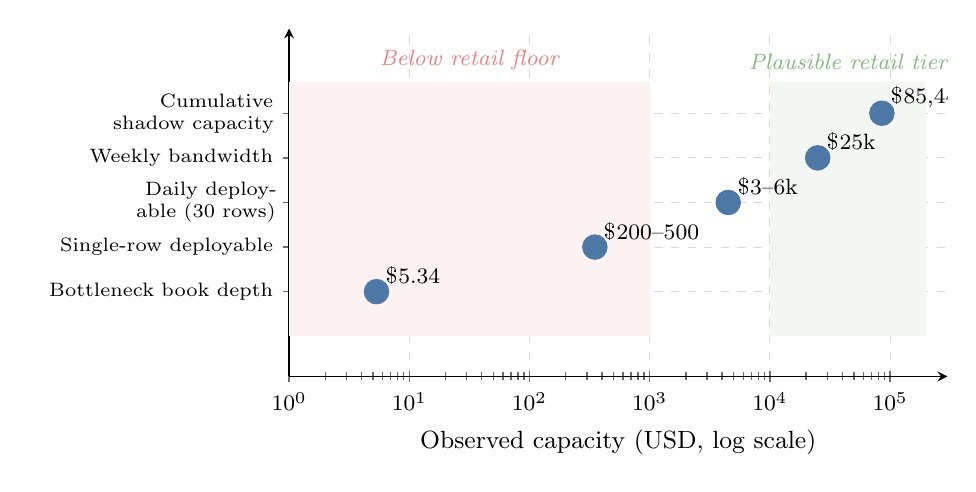
\begin{tikzpicture}
\begin{axis}[
  width=0.82\textwidth, height=6cm,
  xmode=log,
  xmin=1, xmax=300000,
  xlabel={Observed capacity (USD, log scale)},
  ymin=0, ymax=6,
  ytick={1,2,3,4,5},
  yticklabels={Bottleneck book depth, Single-row deployable, Daily deployable (30 rows), Weekly bandwidth, Cumulative shadow capacity},
  yticklabel style={font=\scriptsize, align=right, text width=3.0cm},
  axis y line=left, axis x line=bottom,
  xmajorgrids=true, xminorgrids=false,
  enlarge y limits=0.15,
]
\path[fill=abelred!8] (axis cs:1,0) rectangle (axis cs:1000,5.7);
\node[anchor=south, font=\footnotesize\itshape, color=abelred!75] at (axis cs:31.6,5.75) {Below retail floor};
\path[fill=abelgreen!8] (axis cs:10000,0) rectangle (axis cs:200000,5.7);
\node[anchor=south, font=\footnotesize\itshape, color=abelgreen!75] at (axis cs:44721,5.75) {Plausible retail tier};
\addplot+[only marks, mark=*, mark size=4pt, abelblue]
  coordinates {(5.34,1) (350,2) (4500,3) (25000,4) (85446.78,5)};
\node[anchor=west, font=\footnotesize] at (axis cs:5.34,1.35) {\$5.34};
\node[anchor=west, font=\footnotesize] at (axis cs:350,2.35) {\$200--500};
\node[anchor=west, font=\footnotesize] at (axis cs:4500,3.35) {\$3--6k};
\node[anchor=west, font=\footnotesize] at (axis cs:25000,4.35) {\$25k};
\node[anchor=west, font=\footnotesize] at (axis cs:85446.78,5.35) {\$85,446.78};
\end{axis}
\end{tikzpicture}
\caption{Capacity ladder observed across retail prediction-market routes in the Abel AI Lab corpus. Bottleneck book depth (\$5.34) was repeatedly observed in the crypto-PM probe; single-row deployable size (\$200--500) appears in the LLM-narrative-trade campaign; multi-row daily deployability scales to \$3k--6k after thirty events; the proposed weekly bandwidth (\$25k) is the design budget for Path C; the largest observed shadow-only capacity frontier (\$85,446.78) comes from \texttt{pm-10k50k-profit} but lacks priors and live execution. Below \$1k is the retail floor at which fixed costs and variance dominate; above \$10k is plausible retail tier when many concurrent rows can run.}
\label{fig:capacity-ladder}
\end{figure}

Crypto-pm-probe illustrates the small-cycle version. A route could look attractive on gross spread, but the bottleneck side of the book carried only a few dollars of fillable size: eleven contracts at a best NO price near \$0.485, or roughly \$5.34 of executable depth.\footnote{Quote [E16] sourced from \texttt{crypto-pm-probe/round-2/peer-A.txt:L74}.} Peer review therefore treated the advertised 23.6\% spread as a fillability failure capped at \$5.34 rather than as a scalable strategy.\footnote{Quote [E17] sourced from \texttt{crypto-pm-probe/round-2/peer-A.txt:L74}.} The next gate was correspondingly mechanical: reject rows where the smaller of inside-YES and inside-NO dollar depth is below \$100.\footnote{Quote [E18] sourced from \texttt{crypto-pm-probe/round-2/peer-A.txt:L75}.} That is not a rounding issue. It changes the object being evaluated from a portfolio strategy to a market microstructure curiosity.

The lesson is capacity-weighted edge. A 23.6\% spread on \$5.34 is not comparable to a 200 bps signal on \$50k. The former can be real and still irrelevant to a retail pool that targets greater-than-\$1k-per-month profit. This is the same adverse-selection logic that standard market microstructure applies to spread capture. \textcite{Glosten1985BidAskTransactionPrices} explain why bid and ask quotes embed the risk of informed trading; \textcite{Easley1996LiquidityInformation} connect liquidity and information when trading is infrequent; \textcite{Stoll1989BidAskSpreadComponents} separates spread components that cannot be treated as free expected return. The displayed price is economically meaningful only when the trader can fill enough size without moving into worse levels or being selected against by better-informed flow. Prediction-market order-book studies in the reference set, including \cite{Dubach2026AnatDece}, are useful background for that distinction.

llm-narrative-trade-0125 exposes the pre-PnL version. Peer review found a real CLOB book for one striking gap, with bid 0.51, ask 0.52, and five-figure displayed inside size on both YES and NO.\footnote{Quote [E19] sourced from \texttt{llm-narrative-trade/round-2/peer-A.txt:L82}.} The immediately tradeable amount was still retail-small: roughly \$50--100 inside size per fill before slippage past 0.52 to 0.55, or about \$200--500 deployable on that row.\footnote{Quote [E20] sourced from \texttt{llm-narrative-trade/round-2/peer-A.txt:L83}.} Scaling to a daily \$3k--6k capacity required \$50--200 fills across more than thirty events, so the same evidence that falsified stale Gamma metadata also made capacity an explicit multi-row condition.\footnote{Quote [E21] sourced from \texttt{llm-narrative-trade/round-2/peer-A.txt:L88}.}

Those numbers define the \$10k-to-\$100k transition. At \$10k, a \$3k daily inflow can matter if holding periods are short and realized edge is large. At \$25k, the same inflow is already a utilization problem unless many rows can run in parallel. At \$100k, the route either scales opportunity count by roughly an order of magnitude, keeps orders resting for many days, or moves into larger markets where the LLM edge is less likely to survive.

Bankruptcy-operator-0125 contributes a different capacity failure: access depth rather than book depth. The available public-scrape evidence did not expose enough claim-specific executable inventory; the first peer review found only two rows in the claims log and summarized the dataset as sparse.\footnote{Quote [E22] sourced from \texttt{bankruptcy-operator/round-1/peer-B.txt:L94-L95}.}\footnote{Quote [E23] sourced from \texttt{bankruptcy-operator/round-1/peer-B.txt:L97-L98}.} A later review made the deployability boundary explicit: public web scraping did not expose enough live, actionable, claim-specific inventory for a \$100k deployer.\footnote{Quote [E24] sourced from \texttt{bankruptcy-operator/round-2/peer-B.txt:L25}.} Aggregate pricing pages and plan snippets can support a desk memo, but a \$100k deployer needs class, minimum size, transfer mechanics, fees, and actual broker quotes.

The bankruptcy route shows why capacity is not only book depth. It can also be access depth. If the true opportunity requires broker relationships, claim-transfer paperwork, KYC, minimum ticket sizes, and class-specific legal diligence, then a public scraper has not reached deployable capacity even when it reaches real documents. The route may still exist as an operator business, but it is not the same as a low-touch LLM trading system.

PM-10k50k-profit gives the most constructive counterexample. One round verified cumulative-to-50bps capacity of \$85,446.78 across four accepted candidates, about \$21k on average, and peer review called that scale plausible for mid-tier Polymarket liquidity.\footnote{Quote [E25] sourced from \texttt{pm-10k50k-profit/round-1/peer-A.txt:L35}.} The same review kept the accounting honest by excluding candidate capacity from pool-value delta, preventing phantom pool growth from unfilled depth.\footnote{Quote [E26] sourced from \texttt{pm-10k50k-profit/round-1/peer-A.txt:L36}.} Later peer review verified that the frontier was shadow-only: forty rows, eight deployable candidates, fifteen capacity-deployable rows, thirty prior-deployable rows, zero positions appended, and zero live orders.\footnote{Quote [E27] sourced from \texttt{pm-10k50k-profit/round-20/peer-B.txt:L17}.} Deployable rows still needed current evidence and priors before paper entry.

This counterexample matters because it prevents the section from claiming that retail capacity is always tiny. Some mid-tier Polymarket rows can display five-figure capacity within a slippage band. The missing piece is simultaneous evidence: official source routeability, fresh market data, a prior strong enough to clear the raw-prior ceiling, and a paper execution path. Capacity alone does not become PnL, but capacity measured separately keeps the system honest.

Cross-platform-pilot-b adds the venue-matching version of the ceiling. Cross-venue spread ideas are attractive precisely because they appear to escape a single venue's order-book limits. The campaign evidence instead pointed to matching failure and operational capacity near zero for the tested route. A cross-venue mechanism proves shared event semantics, venue access, fee models, withdrawal and settlement latency, and both-side depth before it can claim scale.

The pool-tier map follows from those cases. Around \$1k, the right question is whether the mechanism survives a smoke test without hidden fees or obvious leakage. Around \$10k, the question becomes whether opportunity frequency prevents idle capital. Around \$25k, row independence and fill sequencing begin to matter because a few small fills cannot drive returns. Around \$100k, the route reports inside size, expected hold time, fee drag, settlement status, and post-fee PnL in one ledger. Beyond \$1M, the evidence needed is institutional: queue priority, rebate and fee tiers, API latency, private inventory, and principal-book risk.

The recurring peer pattern is that idea generation was rarely the binding constraint. The binding constraint was turning an idea into fresh, fillable, settlement-grounded, capacity-weighted deployment. A route that cannot report inside size, expected hold time, fee drag, and settlement status is not yet a retail-bankroll route. These are blockers, not details for later optimization.

The retail tier is therefore caught between fee floor and capacity ceiling. The most mechanical opportunities are too small, the liquid markets are too efficient, and LLM-sourced priors require an uncertainty buffer large enough to erase many apparent edges. Capacity and edge have to be evaluated as one object from the first round, not after a nominal alpha has already been declared.

Across the 11 trading-focused campaigns, at least six quantified cycle or row economics below the intended deployment floor before claiming profit: cross-platform-pilot-b reached 0 of 30 overlap on the reference corpus and therefore \$0 capacity on that target; profit search ended at \$0.32/day on a \$100k pool; crypto-pm-probe exposed a \$5.34 bottleneck; llm-narrative-trade measured roughly \$200 to \$500 deployable on the sharpest single row and \$3k to \$6k daily deployability only after 30-plus rows; bankruptcy-operator found only two claim rows and no executable \$100k inventory; pm-10k50k-profit found \$85,446.78 of cumulative-to-50bps candidate capacity but kept it shadow-only until evidence and priors could be attached. Capacity evidence was therefore not absent; it repeatedly arrived before profit evidence and forced the route to stay below live-capital language.

\section{Anchoring Uncertainty as Trading Constraint}
\label{sec:anchoring-uncertainty-as-trading-constraint}
An LLM prior near the market price is not independent just because the system labels it "prior." Anchoring uncertainty is a trading constraint, narrower than a claim about LLM truthfulness and narrower than a claim about market efficiency.

MarketAnchor v0.1.2 measured consensus-anchor sensitivity in one stored prediction-market forecasting run. The headline mean net signed drift was 256.73 probability basis points across 75 triplets, with high-anchor movement larger than low-anchor movement.

The sister paper's disclaimer is reproduced here in substance because it is central to proper use: the statistic is not expected-return bps, not realized alpha, not calibration error, and not trading profit without a separate portfolio model. The fifth disclaimer is explicit: it is not a forecast-accuracy result. MarketAnchor measures how forecasts move under anchor framing; it does not say whether the unanchored forecasts resolve correctly.

Paper 2 uses that result only for one proposition: if a prompt exposes market consensus and then asks an LLM for an independent prior, the elicited prior can be contaminated by the prompt itself.

The trading argument is separate and comes from Paper 2's corpus. If a strategy's apparent LLM-prior edge is below roughly 500 bps, and if the prior was elicited near market-price or consensus context, the edge is operationally contaminated unless anchor controls are applied.

The 500 bps figure is not borrowed from MarketAnchor as a return threshold. It is a conservative operational buffer over a 256.73 bps descriptive drift and over the narrative-trade observation that ablation deltas can be hundreds of bps.

llm-narrative-trade-0125 shows the applied problem. Market-quote inclusion and omission changed priors, but the resulting gaps mixed signal, source quality, prompt sensitivity, and model nondeterminism.

In R1, the prompt exposed the current market quote before the LLM emitted the prior. The row schema appeared to place the prior timestamp before the market-quote timestamp, but the model had already seen the quote. That is why this paper treats prompt ordering as a semantic constraint, not only a timestamp constraint.

In R2, peer review identified the direction of the effect: with-quote priors moved toward the market quote in seven of eight events. This is more specific than generic sycophancy. It means a model can absorb visible consensus as if it were authoritative evidence and blend it into the prior even when the route needs an independent estimate.

The R2 same-run variance also matters. Peer review reported mean sigma\_without near 5.6 percentage points across three Codex CLI subprocesses. That variance is larger than the 200-bps to 500-bps edge bands that many retail strategies would try to monetize. A single LLM number therefore cannot be treated as a calibrated probability without ensemble and stability checks.

The trading implication is a noise-floor rule. If the measured anchor drift is roughly 256.73 probability bps in the sister artifact, and if the campaign-specific ablations show hundreds or thousands of bps of movement in some rows, a claimed edge near the market has to clear a larger buffer. The paper uses 500 bps as an operational threshold for suspicion, not as a universal profit cutoff.

This buffer is intentionally conservative. It leaves room for a route with a very large source-grounded disagreement, a stable no-quote prior, and enough book depth to survive. It does not leave room for a row where the model saw the market quote, moved toward it, and then reported a 200-bps gap as independent alpha.

The engineering response is paired prompts, anchor-masked priors, source-grounded evidence, ensemble variance reporting, and capacity-weighted backtests. A single LLM prior near a market price is not independent alpha.

The quote bank ties the anchoring constraint to specific prompt and prior failures: regex anchoring in the profit-search route, a scale-level sycophancy diagnosis, and event-level rows where with-quote priors moved closer to the market. The Evidence Locator appendix records the line-level provenance without turning the body into an audit log.

This finding is a constraint, not a kill switch. LLM priors can still be useful as one feature, especially when external evidence is strong and anchor exposure is controlled. The corpus shows that uncontrolled priors are too unstable for small-edge trading claims.

The safest interpretation is operational. The relevant test is whether an LLM-prior trading system keeps its prior materially stable when visible market consensus is hidden, perturbed, or counterbalanced by source-grounded evidence. It also has to show that the stable prior improves the actual trading ledger after fees, spreads, holding periods, and capacity are included.

This is also why MarketAnchor is not used as a substitute for the Paper 2 corpus. The sister artifact supplies a descriptive anchor-sensitivity measurement and the SHA 8968953708979dc2bd2915ec5c0a22c40e730c24d8134470739b7084bec5ca27 for reproducibility. The trading conclusion comes only after the Abelian campaigns expose how prompt sensitivity interacts with source quality, book depth, and realized execution.

\section{Abelian Methodology Contribution}
\label{sec:abelian-methodology-contribution}
What does an adversarial loop actually do for an agentic research program? In this corpus, it turns vague intent into a contract, rejected routes into auditable evidence, and post-hoc confidence into a sequence of attacks that can be counted. The methodology contribution is the empirical formalization of the Abelian adversarial loop: rule \#16 R0 program gates, asymmetric peer policy, mission-thread route memory, commit-gate progress checks, and frame-break protocol.

The earliest observed R0 program-gate artifact in this corpus is cross-platform-pilot-b at 2026-05-04T01:01:07Z. The methodology timeline identifies the file \texttt{round-0/program-peer-challenge.txt} and records UTC mtime \texttt{2026-05-04T01:01:07.208905+00:00}. Before that point, most campaigns had adversarial review after mutation rather than before launch.

The R0 gate hardens the contract before the loop spends its first real round. The program states the target, eval, metric, budget, files in scope, data gates, and stop conditions; the baseline eval runs before mutation; a program-peer challenge attacks the contract before R1 starts; the contract hash records the launch boundary; and the TTY confirmation records that the human operator accepted it. The steps are procedural, but their effect is empirical: they make pre-launch ambiguity visible.

The gate's value is not that it guarantees success. Its value is that it makes launch defects countable before a round spends engineering time on a fuzzy target, an unverifiable metric, or a borrowed source of authority. In this corpus, plan-level attacks often mattered more than code-level attacks because the route could fail before any implementation existed.

Path C records the clearest R0 trajectory. The initial challenge found 18 attacks across target, eval, metric, scope, and borrowed-authority classes. The second version narrowed the remaining blockers to 3. The third version left 1 residual issue. The fourth version reached 0 launch blockers and permitted R1.

The Path C attack sequence was not cosmetic. The early attacks forced the program to specify EDGAR form coverage, evidence-grounded extraction, special-situation tradeability, cost limits, and how confidence would be interpreted. R1 still failed on implementation, but it failed against a more explicit contract. That difference is methodologically important: the peer review could say exactly which promises were broken.

The Path C per-round meaning is visible in the contraction. The 18-attack round said the program was not ready to launch because the parent target, eval semantics, evidence grounding, and routeability gates were under-specified. The 3-attack round meant the main shape was now testable but still had blocking ambiguities. The 1-attack round meant a single residual launch issue remained. The 0-attack round did not certify profit; it certified that R1 could fail against a named contract.

Paper 2 records a longer R0 trajectory. The prompt-side sequence produced 21 attacks, then 6, then 4, then 3, then 1 before R1 extraction. The later rounds narrowed the paper target from a vague retrospective into a corpus-bound manuscript with line-count, citation, schema, AI-disclosure, and arXiv-verification gates.

Figure~\ref{fig:r0-trajectory} plots those two R0 attack-reduction trajectories.

\begin{figure}[t]
\centering
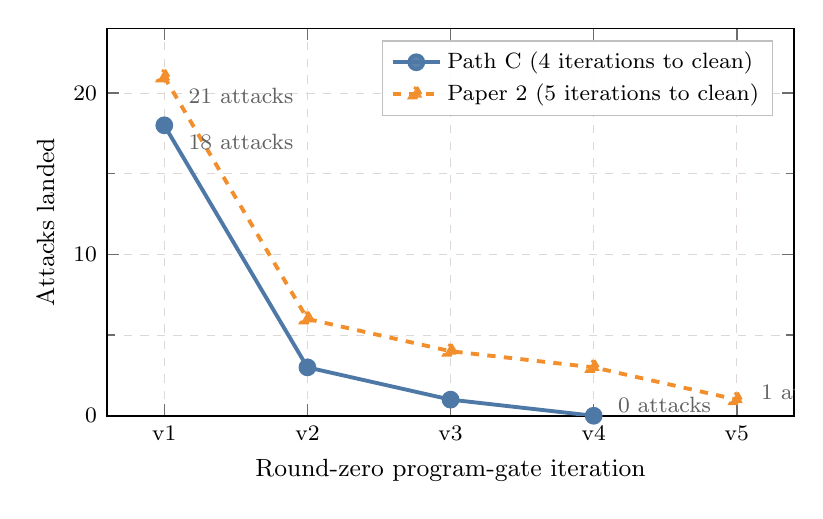
\begin{tikzpicture}
\begin{axis}[
  width=0.85\textwidth, height=6.5cm,
  xlabel={Round-zero program-gate iteration},
  ylabel={Attacks landed},
  xtick={1,2,3,4,5},
  xticklabels={v1, v2, v3, v4, v5},
  ymin=0, ymax=24,
  ymajorgrids=true, yminorgrids=true,
  minor y tick num=1,
  legend pos=north east,
  legend cell align=left,
]
\addplot+[mark=*, abelblue, line width=1.4pt]
  coordinates {(1,18) (2,3) (3,1) (4,0)};
\addlegendentry{Path C (4 iterations to clean)}
\addplot+[mark=triangle*, abelorange, line width=1.4pt, dashed]
  coordinates {(1,21) (2,6) (3,4) (4,3) (5,1)};
\addlegendentry{Paper 2 (5 iterations to clean)}
\node[font=\footnotesize, color=abeldark!75, anchor=west] at (axis cs:1.1, 17) {18 attacks};
\node[font=\footnotesize, color=abeldark!75, anchor=west] at (axis cs:4.1, 0.7) {0 attacks};
\node[font=\footnotesize, color=abeldark!75, anchor=west] at (axis cs:1.1, 19.8) {21 attacks};
\node[font=\footnotesize, color=abeldark!75, anchor=west] at (axis cs:5.1, 1.5) {1 attack};
\end{axis}
\end{tikzpicture}
\caption{Round-zero attack-reduction trajectory across two pre-registered campaigns. Path C narrowed 18 attacks to 0 across four program-gate iterations; Paper 2 narrowed 21 to 1 across five iterations before R1 implementation. Each iteration costs roughly five minutes of program-peer-challenge time and saves roughly half an hour of R1 implementation burn per blocker-or-major attack caught.}
\label{fig:r0-trajectory}
\end{figure}

The methodology-self-attack file turns that trajectory into a costed gate record. It contains 21 Paper 2 R0 self-attacks: 3 BLOCKER, 15 MAJOR, and 3 MINOR. The blocker-or-major set includes target parent directories, contradictory section counts, an R1 plan that could leave \texttt{main.md} absent while the eval stayed at zero, unsupported state extraction across 17 campaigns, empty legacy round directories, regex-only citation counting, missing transcript provenance, v0.1.2 borrowed-credit errors, infrastructure/trading scope confusion, and depth/budget mismatch. At a conservative 0.5 hours of R1 burn per blocker-or-major defect, those 18 pre-R1 catches avoided roughly 9 hours of work that would otherwise have produced uncommittable or reviewer-rejected artifacts.

The Paper 2 per-round meaning is different because the artifact is a manuscript rather than a trading scanner. The 21-attack round challenged corpus definition, active-campaign counts, claim scope, citation authority, and whether paper self-attacks could contaminate trading findings. The 6-attack and 4-attack rounds narrowed the target to a data-backed retrospective. The 3-attack round forced clearer evaluation and disclosure. The final 1-attack round left a bounded residual issue before R1 extraction. That sequence is why the paper treats its own construction as methodology evidence.

The Paper 2 trajectory also shows a weakness of eval-only thinking. R2 later scored 100 under the then-current eval while containing many repeated paragraphs. Peer attack identified the padding, and R3 added a uniqueness gate that caps the score at 75 when paragraph uniqueness falls below 0.85. The methodology contribution is therefore not "evals solve quality." It is that adversarial review and evals attack each other.

The asymmetric peer policy is a second method contribution. Claude peer-A is assigned framing, scope policing, reviewer anticipation, and strategic plausibility. Codex peer-B is assigned heavy extraction, transcript mining, recomputation, implementation, and verification. The roles are not symmetric stylistic labels. They expose different failure surfaces.

The asymmetry matters in this paper because peer-A and peer-B caught different classes of defect. Peer-A repeatedly pressed claim scope, reviewer framing, and hidden generalization risks. Peer-B repeatedly pressed file-line provenance, schema validity, duplicated prose, quote-bank quality, and exact eval behavior. A single generic peer role would have been less likely to cover both.

The policy is also bounded. Peer-B does not get to solve reviewer framing by adding more prose without evidence. Peer-A does not get to approve a claim because the story is elegant. Each role has a different way to say no, and the campaign advances only when the selected route survives both kinds of attack.

Mission threads force rejected routes to stay auditable. Each round records the goal paraphrase, candidate routes, selected route, selection reason, metric delta, blocker status, exploration flag, and frame-break count, so a route's silent disappearance becomes a methodological violation rather than a clean restart.

The mission-thread rule is not bureaucracy. It is a guard against invisible p-hacking of the research process. If the model considered a shallow metadata-only route, a prose-only route, or a data-only route, the state file keeps that fact. The selected route then carries a reasoned comparison against alternatives, not a retrospective story that only the winning path was ever available.

The commit gate then asks for goal progress rather than activity. In this paper, that distinction matters because many campaigns produced code, tests, tables, or prompts while still failing to produce profit evidence or tradeable capacity. A round can be technically busy and strategically null. The commit gate keeps that distinction visible.

A profitable-trading campaign therefore cannot count a scanner as progress unless it moves a pool metric, reaches a verified paper-entry gate, or removes a named blocker on the path to that gate. A paper campaign cannot count lines as progress unless they advance a claim with evidence. R2's padding failure is the negative control that makes the rule concrete.

The frame-break protocol matters when repeated rounds converge on no route. It asks the loop to change frame before declaring termination, but it does not permit unlimited scope expansion. A frame break can move from public scraping to broker calls, or from LLM priors to smart-money signals, only if the new frame names a different mechanism and a measurable gate.

Bankruptcy-operator gives an example. The public-scrape route did not expose enough claim-specific capacity. A valid frame break would ask for executable broker quotes and transfer mechanics for named classes. It would not add another generic scraper and call that creativity. The frame break is a disciplined mechanism change.

Path C and Paper 2 also show that R0 gates can be multi-round objects. A single peer challenge is useful, but the stronger pattern is challenge, rewrite, re-challenge, and only then launch. The sequence turns vague disagreement into a counted convergence process. A contract that begins with 21 attacks and launches with 1 residual issue has a visible hardening trajectory.

This differs from conventional human-led adversarial review in one specific way. The review is not only a post-hoc paper critique or a code review checklist. It is a mutation loop with state, evals, route memory, and explicit stop conditions. The paper does not claim this is better than expert human review. It claims the local corpus provides an instrumented record of how such a loop changes research behavior.

The method is also not fully pre-registered for all campaigns. Most analyzed campaigns were born before rule \#16 was routine. Their peer files still contain adversarial critique, but the critique mostly happens after mutation. Path C and Paper 2 are the cleanest examples of pre-launch contract hardening under the R0 gate.

That chronology is why Section 3 separates trading evidence from methodology evidence. A pre-gate campaign can support a claim about a trading mechanism if its artifacts are sourceable and fillable. It cannot support the claim that the route was pre-registered under rule \#16. Conversely, Paper 2 self-attacks can support the methodology contribution while remaining quarantined from cross-campaign trading recurrence counts.

The methodology timeline records this boundary explicitly. It lists the pre-2026-05-04 campaigns as retrospective, identifies the first R0 gate artifact, describes 2026-05-04 adoption, and records the 2026-05-05 spread into Path C and Paper 2. This prevents the paper from smoothing an evolving method into a uniform protocol.

The supporting methodology evidence is therefore distributed across three local artifacts: the timeline, the state files, and the peer transcripts. The timeline proves chronology. The state files prove route memory and metric updates. The peer transcripts prove that attacks were concrete enough to change implementation or claims.

The result is a paper-level contribution rather than merely a lab anecdote. The loop makes failed trading campaigns legible as data, preserves alternatives that did not win, separates infrastructure hardening from profit evidence, and exposes eval gaming when it appears. That combination is the Abelian methodological claim.

The claim is still bounded. The corpus does not prove that Abelian review dominates other research workflows. It does show that in this lab, the method repeatedly found hidden assumptions before live capital, forced route-specific evidence requirements, and made retrospective failures easier to analyze without converting them into heroic success stories.

\section{Discussion}
\label{sec:discussion}
\subsection{Findings Integration}
\label{subsec:findings-integration}
The strongest paper claim is not that LLM trading cannot work. It is that the retail routes that looked easiest for LLMs shared the same trap: LLM-accessible features are usually accessible to other market participants, and LLM-extracted fields can lack source grounding exactly where trading requires it.

The four findings form one mechanism chain. Math-arb saturation covers public price relationships after obvious violations are visible: 8 of 11 trading-focused campaigns explored math-arb-class or adjacent market-structure routes, and 0 of 8 produced sustainable greater-than-\$1k/month evidence after current-data, fillability, and capacity gates. The negative result is balanced by positives: the 327-trade threshold-ladder arsenal was real historical alpha, bydate LP arb survived in tiny size, and cross-platform scans measured real but sub-floor cycle economics.

The ceiling-pin finding covers prompt-accessible or rubric-accessible fields that looked high-confidence without source binding. The n=3 instances are supported by more than 12 direct source rows across llm-deploy, Path C, and llm-narrative-trade. The capacity ceiling then turns "edge" into deployability: the corpus records \$5.34 bottleneck depth, \$200 to \$500 single-row deployability, \$3k to \$6k daily deployability under a 30-row assumption, \$0.32/day public LP-arb capacity on \$100k, and an \$85,446.78 shadow capacity frontier that still lacked priors and current evidence.

Anchoring uncertainty supplies the fourth gate. The narrative-trade campaign shows both positive and negative evidence: prompt engineering moved priors and R3 produced six newly flagged rows, but the same implementation log recorded zero 24-hour PnL rows backfilled. That is an engineering primitive, not realized trading profit.

The route registry completes the integration. Aggregate state counts 228 proposed routes; 135 were rejected, a 59.2\% rejection rate. The recovered JSONL registry holds 225 rows: 45 selected, 135 rejected, and 45 deferred. Quote-bank quality improved too: 40 verbatim rows, eight max per campaign, and peer-B capped at 24 of 40 quotes so cron-fill/ws-cron infrastructure could not dominate the evidence base.

A candidate strategy therefore earns trading language only after it survives current-data falsification, source-grounded extraction, capacity-weighted execution, and anchor-stable prior estimation. Many ideas produced useful research artifacts before clearing all four gates. That is the central evidence, not an embarrassment to hide.

\subsection{Implications for Builders}
\label{subsec:implications-for-builders}
For builders, the findings translate into gate order. Filing-evidence grounding belongs before any confidence score; otherwise the rubric merely reports back the LLM's surface plausibility. If a field cannot return a source span that a verifier can grep, the row is not tradeable. The recovered promoted-route registry contains 10 evidence/source/filing/grounding routes, the repair family Path C needed after its R2 hallucinated pass row.

LLM priors belong behind anchor-masked prompts before any visible market quote or consensus estimate is introduced. With-quote prompts remain useful as diagnostics, but the canonical alpha source is generated, stored, and variance-checked before comparison to the market. Sixteen promoted recovered routes mention priors, quotes, anchors, ablation, or consensus.

Backtests start as capacity-weighted objects. A strategy that clears a probability threshold but fails on depth, fee drag, spread, holding period, or exit latency has not found deployable alpha at the claimed bankroll. Thirty-nine promoted recovered routes mention capacity, backtest, depth, fill, fee, spread, settlement, or PnL. That count is the builder lesson: capacity is part of the first gate.

Adversarial review also has a sample-bias job. It asks whether the route was selected because it was available, whether failed rows were dropped, whether historical violations came from stale snapshots, and whether a live system would have known the same facts at the same time. The rejected pile shows why: high-estimate routes such as multi-connection sharding often lost to lifecycle, watchdog, observability, or blast-radius blockers.

The constructive role for LLMs is still large: source-span retrieval, rule-text normalization, anomaly triage, hypothesis generation, and adversarial review. A trade inherits the LLM output only after a non-LLM gate confirms the relevant source and execution facts.

\subsection{Methodology Generalization}
\label{subsec:methodology-generalization}
Abelian rule \#16's R0 gate is not specific to prediction-market trading. It is a mechanism for agentic research loops where an incorrect launch is expensive: a trade, a production deploy, a benchmark claim, or a public paper.

The empirical record supports testing that broader use. Path C narrowed 18 program-gate attacks to 3, then 1, then 0 before the campaign proceeded. Paper 2 narrowed 21 attacks to 6, then 4, then 3, then 1 before R1 extraction. In both cases, the launch gate caught critical defects before R1 burn: target parents, elastic eval semantics, borrowed citations, scope creep, empty inventory, and evidence-definition mismatch. The methodology timeline records the first observed R0 gate artifact at 2026-05-04T01:01:07.208905+00:00.

Those reductions do not prove future success; they show that pre-mutation challenge catches scope, citation, metric, and evidence defects while they are still cheap to fix. Natural non-trading inheritors are data releases, benchmark construction, infrastructure migration, compliance-sensitive automation, paper submission pipelines, and agentic deploy loops. The right measurement is defects caught before implementation, not only the final score.

\subsection{What Is Not Claimed}
\label{subsec:what-is-not-claimed}
The paper does not claim that prediction markets are efficient; it claims only that the sampled retail routes did not clear the observed gates in this single-lab corpus. It does not claim that LLMs cannot trade; it claims that these LLM-assisted routes did not become sustainable greater-than-\$1k-per-month retail trading systems after adversarial review.

The paper does not claim that n=3 ceiling-pin observations are universal. It does not claim that Abelian methodology guarantees success. It does not claim that MarketAnchor v0.1.2's 256.73 probability-bps drift is tradable, that the unanchored priors were accurate, or that the sister artifact proves realized edge.

The four findings are single-lab, single-period observations. The correct use is a boundary map and an operational checklist, not a theorem about all prediction markets, all LLMs, or all future market regimes.

\section{Limitations}
\label{sec:limitations}
\subsection{Single-Lab, Single-Operator, Single-Period}
\label{subsec:single-lab-single-operator-single-period}
The study is single-lab, single-operator, and single-period. Stephen Wang ran the campaigns at Abel AI Lab in 2026-Q2 using Claude general-purpose Agent and Codex CLI gpt-5.5 xhigh as the main adversarial tools. No independent replication is claimed.

\subsection{Ceiling-Pin Sample Size}
\label{subsec:ceiling-pin-sample-size}
The ceiling-pin count is n=3 cross-mechanism observations, suggestive not structural. The cleanest count is n=2 if a reader requires only extraction systems: llm-deploy and Path C. The n=3 version adds llm-narrative-trade-0125 because the prompt-gate actionability surface is the same defect family, but that inclusion is not a universal law.

\subsection{Stephen-Curated Selection Bias}
\label{subsec:stephen-curated-selection-bias}
The corpus is Stephen-curated and therefore subject to selection bias. It overrepresents strategies that were plausible to one operator at one lab and underrepresents routes outside that operator's attention, access, or taste. The sample is not a random draw from all possible LLM-trading attempts.

\subsection{Campaigns Predating the Formal R0 Gate}
\label{subsec:campaigns-predating-the-formal-r0-gate}
Most campaigns predate the mature rule \#16 R0 gate. They contain adversarial review and state artifacts, but they did not all begin under the same formal pre-mutation contract discipline. This matters because methodology evidence is strongest when the gate is applied before route selection, not reconstructed after the fact.

\subsection{Reproducibility Pending License Confirmation}
\label{subsec:reproducibility-pending-license-confirmation}
Public-source coverage is incomplete at draft time. Some source artifacts are local run files and memory notes. Public release is planned, but the reproducibility package remains pending license confirmation and repository publication. External reviewers without the repository will need the release bundle before they can reproduce the same provenance checks.

\subsection{Four-Active-Day Execution Span}
\label{subsec:four-active-day-execution-span}
The active execution span is short. The inventory covers a 12-calendar-day window, but the actively executed campaign span is four active days: 2026-05-02 through 2026-05-05. Many findings emerged under compressed time pressure, and they may not generalize to slower research programs that revisit routes over weeks or months.

\subsection{LLM-Family Generalization Caveat}
\label{subsec:llm-family-generalization-caveat}
The LLM-family generalization is limited. The observations come from Codex CLI gpt-5.5 xhigh and Claude general-purpose Agent, both from the same broad RLHF-era family of general-purpose assistant models with similar alignment objectives. Findings may differ for base models, Gemini-family systems, open-weight models, Llama, Mistral, domain-finetuned financial models, or deterministic API configurations with seeds; the ceiling-pin failure mode could be amplified or reduced under different RLHF priors.

\subsection{Survivorship Bias}
\label{subsec:survivorship-bias}
The corpus also has survivorship bias. Campaigns that died at R0 gate refusal or before any logged round are not in the active corpus, so the analyzed 13-active-campaign set is biased toward efforts that produced enough artifacts to inspect. Of 17 raw campaign directories, four legacy directories contain eight empty round directories in total: \texttt{bankruptcy-operator}, \texttt{cftc-event-fragmentation}, \texttt{crypto-bankruptcy-claims}, and \texttt{llm-narrative-trade} (\texttt{per-campaign-summary.csv:L15-L18}); they keep the denominator honest but are too empty to support mechanism claims, while ideas that died before creating even an empty round directory remain invisible.

\subsection{Post-Hoc Methodology Rationalization}
\label{subsec:post-hoc-methodology-rationalization}
The methodology claim is partly post-hoc. Abelian rule \#16's R0 gate emerged mid-session, with the first observation recorded at 2026-05-04T01:01:07Z. Path C and Paper 2 are the cleanest examples fully pre-registered under the formal gate; the other 11 active campaigns are analyzed retrospectively. Section 8 is therefore a calibrated methodology contribution, not proof that the whole corpus was designed under the final gate.

\subsection{Eval-Gaming as Internal Lesson}
\label{subsec:eval-gaming-as-internal-lesson}
The eval-gaming caveat is internal and material. The Paper 2 R2 round produced metric=100 with 117 padded paragraphs before peer attack exposed the failure. The updated uniqueness gate is a repair, not proof that future metrics cannot be gamed. Any LLM-output benchmark that scores prose without uniqueness, provenance, and substantive-contribution gates remains gameable, making this both a limitation of the draft process and a concrete methodological lesson for agentic research evaluation.

\section{Open Problems and Future Work}
\label{sec:open-problems-and-future-work}
Can an anchor-controlled LLM prior survive perturbation and still improve a ledger? The next study elicits priors with hidden, visible, counterfactual, and source-grounded market contexts, then tests whether any edge survives the full perturbation set. It reports no-quote canonical priors, with-quote drift, ensemble variance, and realized after-fee PnL separately.

Can special-situation extraction stay high-confidence after the verifier leaves the model's output and checks the filing or rule text itself? A filing or rule field is accepted only when the system returns the source span and the verifier can grep the span before scoring confidence. The next Path C-style run compares output-grep, filing-grep, and human-verified rows, then reports how many high-confidence candidates survive each gate.

Can participant behavior supply a better signal class than model narration? Insider Form 4 and 13F changes, crypto whale flows, unusual options volume, borrow-rate moves, and order-flow imbalance differ from LLM prior extraction because the information source is behavior rather than prose. The probe is timestamped, leak-checked, and capacity-weighted from the start.

The existing corpus contains the motivation but not yet the route registry row for this mechanism. Path C's compound handoff names a future Path D with insider transactions, options flow, or satellite data as a different source class (\texttt{2026-05-05-path-c-1week-probe/COMPOUND\_DOC.md:L60}). That absence is itself a clean open problem: the next route registry needs an explicit participant-behavior lane instead of relying on LLM narration or public price fields.

What makes a cross-venue spread executable rather than merely visible? Cross-platform spread ideas need synchronized fee models, withdrawal and settlement latency, order-book depth, venue-specific fill constraints, and rule-semantics matching before alpha language is warranted. A useful study fails rows independently on each axis rather than reporting a single aggregate spread.

Do ceiling-pins survive a change in model family? The llm-deploy and Path C findings need reruns on base models, Gemini-family models, open-weight Llama and Mistral systems, and domain-finetuned financial models. The experiment tests whether rubric-side and prompt-side ceiling-pins persist when models differ in training, alignment, determinism, and tool-use behavior. Moving from n=3 to a stronger claim requires this replication.

Where does the capacity ladder change once the bankroll leaves retail scale? The paper maps the retail-bankroll transition from \$1k smoke tests to \$100k utilization pressure. It does not map institutional, HFT, or principal-book regimes. A follow-on study separates retail API execution, professional market-making, broker-mediated OTC operation, and principal inventory risk.

\section*{Acknowledgments}
External editorial and methodological feedback from independent paper-review consultations improved metric naming, R1/R2 protocol stratification, contract-cluster sensitivity analysis, AI/tool author-policy disclosure, and related-work coverage before submission.

\printbibliography

\appendix
\section{Evidence Locator}
\label{app:evidence-locator}

\begingroup
\footnotesize
\setlength{\tabcolsep}{3pt}
\renewcommand{\arraystretch}{1.12}
\begin{longtable}{@{}>{\raggedright\arraybackslash}p{0.07\textwidth}>{\raggedright\arraybackslash}p{0.30\textwidth}>{\raggedright\arraybackslash}p{0.55\textwidth}@{}}
\caption{Line-level locator for integrated evidence quotes and quote-bank entries.}
\label{tab:evidence-locator}\\
\toprule
\textbf{ID} & \textbf{Source} & \textbf{Verbatim Quote} \\
\midrule
\endfirsthead
\toprule
\textbf{ID} & \textbf{Source} & \textbf{Verbatim Quote} \\
\midrule
\endhead
E1 & \path{llm-deploy-10k/round-1/peer-A.txt:L16} & 0/18 events were skipped on `rule\_reader\_confidence < 80` --- every event scored 100. This is a ceiling-pinned signal \\
E2 & \path{llm-deploy-10k/round-1/peer-A.txt:L39} & Rubric is `25 x n\_extracted\_fields` and PM gamma metadata trivially has all 4 fields \\
E3 & \path{llm-deploy-10k/COMPOUND_DOC.md:L22} & passed\_rule\_reader (>=80 confidence) | 18 (100\%) \\
E4 & \path{llm-deploy-10k/COMPOUND_DOC.md:L4} & 18-event historical backtest shows -23\% net on \$4250 deployed with hit\_rate 41.2\% \\
E5 & \path{path-c-1week-probe/round-1/peer-A.txt:L8} & R1 ships SAME ceiling-pin defect class as llm-deploy V3 (regulatory + consideration\_quant axes auto-credit on truthy-string) \\
E6 & \path{path-c-1week-probe/round-1/peer-A.txt:L39} & regulatory\_agency axis ceiling-pinned: scoring.py:10-11 accepts ANY non-empty string \\
E7 & \path{path-c-1week-probe/round-1/peer-A.txt:L40} & consideration\_quant axis ceiling-pinned: scoring.py:5 accepts ANY non-empty string \\
E8 & \path{path-c-1week-probe/round-2/peer-A.txt:L8} & the SOLE high-confidence row is a hallucination on 3 fields \\
E9 & \path{path-c-1week-probe/round-2/peer-A.txt:L41} & the LLM fabricated "none required" in the JSON output \\
E10 & \path{path-c-1week-probe/round-2/peer-A.txt:L63} & Quality-adjusted >=80 rate = 0/18 today \\
E11 & \path{llm-narrative-trade/round-1/peer-A.txt:L15} & Engine prompt embeds market\_quote BEFORE asking for prior \\
E12 & \path{llm-narrative-trade/round-1/peer-A.txt:L55} & the LLM is NOT citing the SOURCE BUNDLE. It's citing FACTS FROM TRAINING DATA \\
E13 & \path{llm-narrative-trade/round-2/peer-A.txt:L24} & Signal: 7/8 events show with-quote prior pulled toward market regardless of sign \\
E14 & \path{llm-narrative-trade/round-3/codex-implement.txt:L13015} & Updated with\_quote=False prompt to explicitly prohibit market anchoring. \\
E15 & \path{llm-narrative-trade/round-3/codex-implement.txt:L13047} & events\_with\_24h\_pnl\_backfilled: 0 \\
E16 & \path{crypto-pm-probe/round-2/peer-A.txt:L74} & 11 contracts at NO best price approximately \$0.485 = \textasciitilde{}\$5.34 of fillable NO depth \\
E17 & \path{crypto-pm-probe/round-2/peer-A.txt:L74} & AXIS 2 FAILS FILLABILITY --- the alleged 23.6\% spread is CAPACITY <= \$5.34 \\
E18 & \path{crypto-pm-probe/round-2/peer-A.txt:L75} & R3 must: (a) reject rows where min(inside\_size\_yes\_dollars, inside\_size\_no\_dollars) < \$100 \\
E19 & \path{llm-narrative-trade/round-2/peer-A.txt:L82} & CLOB book: bid=0.51, ask=0.52, inside\_size\_yes=11130 USDC, inside\_size\_no=16052 USDC \\
E20 & \path{llm-narrative-trade/round-2/peer-A.txt:L83} & at \$50-100 inside-size per fill before slippage past 0.52->0.55 = \textasciitilde{}\$200-500 deployable \\
E21 & \path{llm-narrative-trade/round-2/peer-A.txt:L88} & At \$50-200 per-event inside-size and 30+ events for statistical power, daily deployable approximately \$3-6k \\
E22 & \path{bankruptcy-operator/round-1/peer-B.txt:L94-L95} & The claims\_log has only two rows. \\
E23 & \path{bankruptcy-operator/round-1/peer-B.txt:L97-L98} & the dataset is sparse \\
E24 & \path{bankruptcy-operator/round-2/peer-B.txt:L25} & public web scraping does not expose enough live, actionable, claim-specific inventory for a \$100k deployer \\
E25 & \path{pm-10k50k-profit/round-1/peer-A.txt:L35} & accepted\_capacity\_usd=85446.78 across 4 accepts (\textasciitilde{}\$21k avg) is plausible for PM mid-tier liquidity \\
E26 & \path{pm-10k50k-profit/round-1/peer-A.txt:L36} & capacity stats excluded from pool\_value\_delta\_usd --- prevents the "phantom pool growth from unfilled candidate depth" inflation class \\
E27 & \path{pm-10k50k-profit/round-20/peer-B.txt:L17} & 40 rows, 8 deployable candidates, 15 capacity-deployable rows, 30 required-prior-deployable rows, 0 positions appended, 0 live orders \\
Q001 & \path{cron-fill-grounded-truth/round-1/peer-B.txt:L60-L60} & Cite: math\_arb\_scanner.py:1227-1230 rejects any mlspread row whose `side` contradicts `line`; ws/cron\_full\_replay.py:389-399 trusts `row["side"]` a... \\
Q002 & \path{ws-cron-alignment/round-1/peer-A.txt:L39-L39} & Why this matters: the 64-cid gap is the OLD math-arb-friendly subscription \\
Q003 & \path{ws-cron-alignment/round-1/peer-A.txt:L171-L171} & [MINOR-3] bydate low-n: cron\_resolved\_7d=4. Computing pe\_alignment on n=4 \\
Q004 & \path{ws-cron-alignment/round-2/peer-B.txt:L19-L19} & - `rg -n "Did not write|pair-aware|watchdog|math-arb-friendly|cron-flagged|hybrid" round-2/peer-A.txt` returns peer-A lines 7, 17-26, 33-45, 85-90,... \\
Q005 & \path{ws-cron-alignment/round-2/peer-B.txt:L21-L21} & - `rg -n "ladder\_audit\_rows\_last\_7d | n\_ladder\_pairs\_in\_master | n\_ladder\_pairs\_both\_subscribed | structural\_silence..." \\
Q006 & \path{ws-cron-alignment/round-2/peer-B.txt:L22-L22} & - `rg -n "reconnect attempt|watchdog|subscribing" /tmp/pmpt-ws-paper-soak.log | tail -30` returns cron-flagged watchdog attempts 3-12 and then math... \\
Q007 & \path{cron-fill-grounded-truth/round-1/peer-B.txt:L105-L105} & rationale: attacks look-ahead/latency-skew while preserving R56-style price matching as a lower-confidence fallback \\
Q008 & \path{ws-cron-alignment/round-1/peer-A.txt:L63-L63} & [MAJOR-2] token-cap-truncation-fairness: structural ceiling unsurfaced. \\
Q009 & \path{ws-cron-alignment/round-1/peer-A.txt:L70-L70} & is 220 cids. Therefore the THEORETICAL CEILING of subscribe\_alignment is: \\
Q010 & \path{ws-cron-alignment/round-1/peer-A.txt:L78-L78} & working but operating at 9\% of the structural ceiling." Both are bad, but \\
Q011 & \path{llm-narrative-trade/round-2/peer-B.txt:L47-L47} & 32. Thus sycophancy/anchoring is confirmed as a structural risk, but the interpretation should be "market quote pulls the prior toward itself", not... \\
Q012 & \path{pm-5k10k-profit/round-1/peer-B.txt:L31-L31} & def size\_position(llm\_prior, market\_quote, rule\_reader\_confidence, pool\_size\_usd): \\
Q013 & \path{cron-fill-grounded-truth/round-1/peer-B.txt:L103-L103} & mechanism: compare book depth at scanner observation timestamp or a declared symmetric tolerance window instead of any time until last\_seen \\
Q014 & \path{profit-search/round-1/peer-B.txt:L59-L59} & capacity\_at\_pool\_pct = inside\_size $\times$ 0.50 / 100000. Real Polymarket mechanics: \\
Q015 & \path{profit-search/round-1/peer-B.txt:L89-L89} & of 0xdfc8. capacity\_at\_pool\_pct sum (0.0038\% + 0.0232\% = 0.027\%) is the \\
Q016 & \path{profit-search/round-1/peer-B.txt:L91-L91} & positions before computing capacity, OR note in inventory that 27+31 capacities \\
Q017 & \path{profit-search/round-1/peer-B.txt:L108-L108} & B. **Shared 0xdfc8 capacity double-count**. Aggregate per-cid net positions \\
Q018 & \path{profit-search/round-1/peer-B.txt:L116-L116} & itself is honest; downstream accounting (capacity, walk-deeper) is incomplete. \\
Q019 & \path{profit-search/round-1/peer-B.txt:L26-L26} & 'NOT\_FEASIBLE' $\to$ None (anchor `\textasciicircum{}` is what excludes the negative case) \\
Q020 & \path{llm-narrative-trade/round-2/peer-A.txt:L15-L15} & D2 (sycophancy / authority-by-citation): CONFIRMED at scale. Direction inspection per-event: \\
Q021 & \path{llm-narrative-trade/round-2/peer-A.txt:L16-L16} & - G7 leader: market=0.76, mean\_with=0.69, mean\_without=0.23 $\to$ with closer to market by 46pp. ANCHOR-IN. \\
Q022 & \path{llm-narrative-trade/round-2/peer-A.txt:L17-L17} & - Trump/GTA 540820: market=0.515, mean\_with=0.235, mean\_without=0.068 $\to$ with closer by 17pp. ANCHOR-IN. \\
Q023 & \path{llm-narrative-trade/round-2/peer-A.txt:L18-L18} & - BTC 150k: market=0.0135, mean\_with=0.020, mean\_without=0.063 $\to$ with closer by 4.4pp. ANCHOR-IN (toward 0). \\
Q024 & \path{llm-narrative-trade/round-2/peer-A.txt:L19-L19} & - Pistons: market=0.0605, mean\_with=0.066, mean\_without=0.133 $\to$ with closer by 6.7pp. ANCHOR-IN (toward 0). \\
Q025 & \path{cron-fill-grounded-truth/round-1/peer-B.txt:L47-L47} & [research-class R4 look-ahead, research-class R5 target-leakage, book-depth-fillability-extension latency-skew-between-scanner-observation-T-and-bo... \\
Q026 & \path{cron-fill-grounded-truth/round-1/peer-B.txt:L59-L59} & [research-class R5 target-leakage, specific-gap mlspread-side-flip, replication-failure] \\
Q027 & \path{cron-fill-grounded-truth/round-1/peer-B.txt:L78-L78} & Cite: eval.sh:18 defaults `ASOF` to `date -u`; ws/cron\_full\_replay.py:968 uses `\_parse\_asof(asof)`, and R56 `\_parse\_asof` at ws/cron\_postfix\_ws\_rep... \\
Q028 & \path{cross-platform-pilot-b/round-1/peer-B.txt:L22-L22} & Read-only HTTP GETs, no shared state in connector module. **n/a-this-target**. \\
Q029 & \path{profit-search/round-1/peer-B.txt:L7-L7} & verdict: PRODUCTIVE-DISAGREEMENT --- schema/eval/regex/fee-netting sound; \$0.50 capital model + shared 0xdfc8 double-count + missing walk-deeper rows... \\
Q030 & \path{profit-search/round-1/peer-B.txt:L32-L32} & \textasciitilde{}23.93 h until both entries auto-reject. eval.sh line 40-58 enforces this. \\
Q031 & \path{crypto-pm-probe/round-1/peer-B.txt:L8-L8} & verdict: flags-for-r2 | R1 scanner is keepable as a skeleton, but R2 must replace testnet fair value, lifecycle handling, book validation, and sche... \\
Q032 & \path{crypto-pm-probe/round-1/peer-B.txt:L16-L16} & This is n/a-this-target for secrets, but it means R2 cannot silently add private exchange APIs without adding auth and redaction gates. \\
Q033 & \path{crypto-pm-probe/round-1/peer-B.txt:L20-L20} & Runnable X: monkeypatch `get\_json` to return `\{"bids":[\{"price":"NaN"\}],"asks":[\{"price":"1"\}]\}` and `float("NaN")` flows into JSON as `NaN`, which... \\
Q034 & \path{crypto-pm-probe/round-1/peer-B.txt:L25-L25} & Grep-able X: `rg -n "flock|fcntl|lock|rename|fsync" ws/crypto\_pm\_scanner.py abelian/programs/crypto-pm-probe-eval.sh` finds no locking protocol. \\
Q035 & \path{llm-narrative-trade/round-2/peer-A.txt:L20-L20} & - Senate: market=0.495, mean\_with=0.437, mean\_without=0.34 $\to$ with closer by 9.7pp. ANCHOR-IN. \\
Q036 & \path{llm-narrative-trade/round-2/peer-A.txt:L21-L21} & - Canada Cup: market=0.49, mean\_with=0.557, mean\_without=0.58 $\to$ with closer by 2.3pp. ANCHOR-IN (mild). \\
Q037 & \path{pm-10k50k-profit/round-1/peer-A.txt:L21-L21} & - Check: default config now matches probe contract (notional=1000, slippage\_cap=0.03). No silent override path observed in runtime log. \\
Q038 & \path{pm-10k50k-profit/round-1/peer-A.txt:L31-L31} & - Check: tri-state (none|partially|fully) avoids the binary-flip trap that caused the 2026-04-30 false-clear. progress\_class=discovery\_only aligns... \\
Q039 & \path{pm-10k50k-profit/round-1/peer-A.txt:L34-L34} & - Claim: candidate capacity is cumulative ask depth to 50bps; logs capacity\_slippage\_bps and top\_ask\_capacity\_usd. \\
Q040 & \path{pm-10k50k-profit/round-1/peer-A.txt:L36-L36} & - Cross-check: capacity stats excluded from pool\_value\_delta\_usd --- prevents the "phantom pool growth from unfilled candidate depth" inflation class... \\
\bottomrule
\end{longtable}
\endgroup

\section{Reproducibility}
\label{sec:reproducibility}
\begingroup
\small
Primary repository: Abel AI Lab polymarket\_paper\_trade-ws (analysis code under ws/, Abelian campaigns under abelian/runs/).

Git commit analyzed: e361f9903a0e1f5fd06ee218950c662dbe1190f1

Cross-campaign aggregate file: \path{docs/research/paper-2-llm-extraction-and-pm-saturation/cross-campaign-aggregate.json}

Attack registry: \path{docs/research/paper-2-llm-extraction-and-pm-saturation/anc/attack-registry.jsonl}

Methodology self-attacks: \path{docs/research/paper-2-llm-extraction-and-pm-saturation/anc/methodology-self-attacks.jsonl}

Alternative-route registry: \path{docs/research/paper-2-llm-extraction-and-pm-saturation/anc/alternative-routes.jsonl}

Quote bank: \path{docs/research/paper-2-llm-extraction-and-pm-saturation/anc/quote-bank.jsonl}

MarketAnchor v0.1.2 cross-cite SHA256: \texttt{8968953708979dc2\allowbreak bd2915ec5c0a22c4\allowbreak 0e730c24d8134470\allowbreak 739b7084bec5ca27}

Public release plan: GitHub repository under Abel AI Lab plus Zenodo DOI for archival; release pending license confirmation. Estimated release date: within 2 weeks of arXiv submission.
\endgroup
\end{document}
